\begin{abstract}

Cytolytic T cell responses are predicted to be biased towards membrane proteins. 
Because the peptide-binding grooves of most haplotypes 
of histocompatibility complex class I (MHC-I) are relatively hydrophobic, 
peptide fragments derived from transmembrane helices (TMHs) 
are predicted to be presented more often than expected based on their abundance.
However, the physiological reason of why membrane proteins might be 
over-presented is unclear
In this study, we show the TMHs are evolutionarily more conserved, 
as relatively less single nucleotide polymorphisms (SNPs) 
are present in TMH-coding chromosomal regions 
compared to regions coding for extracellular and cytosolic protein regions. 
Moreover, we show that the over-presentation of TMH-derived peptides is 
likely general, as it is predicted for diverse microbial pathogens 
and for both MHC-I and MHC-II.
Thus, our findings suggest that T cells might respond 
more to membrane proteins, because these are evolutionary more conserved.
We speculate that TMHs might be less prone of the escape mutations 
that enable pathogens to evade T cell responses.

\end{abstract}

{\bf Keywords:} antigen presentation, membrane proteins, bioinformatics, 
adaptive immunity, transmembrane domain, transmembrane helix, 
epitopes, T lymphocyte, MHC-I, MHC-II, evolutionary conservation

%%%%%%%%%%%%%%%%%%%%%%%%%%%%%%%%%%%%%%%%%%%%%%%%%%%%%%%%%%%%%%%%%%%%%%%%%%%%%%%%
\section{Introduction}
%%%%%%%%%%%%%%%%%%%%%%%%%%%%%%%%%%%%%%%%%%%%%%%%%%%%%%%%%%%%%%%%%%%%%%%%%%%%%%%%

% \paragraph{Immune response}

Our immune system fights microbial pathogens, 
such as fungi, bacteria or viruses. 
An important part of the acquired immune response, 
that develops specialized and more effective recognition of pathogens, 
are T cells which recognize peptides derived from the pathogens 
by use of Major Histocompatibility Complexes (MHC). 

% GvdB: Not really relevant. You don’t really need to explain the role of DCs. 
% What is far more important is the concept of what an MHC is: 
% a protein complex that contains a fold, called the peptide-binding groove, 
% which presents peptides. Also immediately explain that MHC-I 
% presents peptides of about 9-amino acids in length to cytolytic T cells, 
% whereas MHC-II presents longer peptides to helper T cells.

% \paragraph{Classification of HLA}

Any individual's immune system detects only a fraction of all possible
peptide fragments.
For humans, the MHC proteins are encoded by the
HLA (Human Leukocyte Antigens) genes.
There are three genes encoding for MHC-I, which are HLA-A, HLA-B and HLA-C,
for MHC-II there are three major genes, which are HLA-DR, HLA-DQ, HLA-DP.
Each MHC complex can only bind a subset of all possible peptides.
For example, HLA-A and HLA-B have no overlap in which
peptides they bind (\cite{lund2004definition}).
The HLA region of humans is highly polymorphic, with hundreds 
to thousands of different alleles, 
and each different HLA gene is called 
an MHC haplotype (\cite{marsh2010nomenclature}).

% \paragraph{HLAs increase detection range}

Because of these multiple and highly polymorphic MHC genes,
the number of pathogenic peptides that can be detected is increased,
as a wide variety of MHCs will be expressed,
each presenting their own subset of epitopes.
It is believed that this improves immunity at the population level, 
as mutations in a protein that disrupt a particular MHC presentation, 
so-called escape mutations, 
will not affect MHC presentation for all haplotypes \richel{Reference needed}.

% \paragraph{Epitope prediction}

Much studies are aimed at determining which peptides are presented in MHC 
and will result in an immune response, 
as this will for instance aid the design of vaccines. 
These studies have led to the development 
of very reliable prediction algorithms 
that allows for in silico predictions 
of the binding affinities of peptides (\cite{larsen2010identification,schellens2008unanticipated,tang2011genome}).
 
% \paragraph{TMHs}

Using these prediction algorithms, 
we recently showed that peptides derived 
from transmembrane helices (TMHs) 
are predicted to be more frequently presented by MHC-I 
than expected based on their abundance (\cite{bianchi2017}). 
Moreover, we showed that some well-known immunodominant peptides stem from TMHs. 

This over-presentation is entirely explained by the fact 
that the peptide-binding groove of most MHC-I haplotypes 
is relatively hydrophobic, 
and therefore hydrophobic peptides have a higher affinity 
than hydrophilic peptides. 

Transmembrane helices (TMHs) are hydrophobic 
as they need to span the hydrophobic lipid bilayer of cellular membranes, 
and they consist of an alpha helix of usually 23 amino acids. 
TMHs are common structures in the proteins of humans and pathogens. 
Different TMH prediction tools estimate
that 15-39% of the proteins in humans 
contain at least one TMH (\cite{ahram2006estimation}). 
TMHs can also be predicted from a protein sequence 
with high accuracy by bioinformatics approaches (\cite{krogh2001predicting,bianchi2017,kall2004combined,arai2004conpred,jones2007improving,klammer2009metatm,wang2019efficient}).

However, the physiological reason why peptides derived from TMHs 
would be presented more often than peptides 
stemming from soluble protein regions is unknown. 
One possibility is that the presentation of 
hydrophobic/TMH residues is evolutionary selected for, 
because TMHs are less prone to undergo escape mutation. 
One reason to expect such a reduced 
variability (and hence evolutionary conservation) in TMHs, 
is that these are restricted in their evolution 
by the functional requirement to span a lipid bilayer. 
Due to this, there are constraints in the types of amino acids 
that can be present in the TMH \richel{ref}. 
Therefore, the TMHs of pathogens 
might have a lower chance to develop an escape mutations, 
as many mutations will result in a dysfunctional TMH 
and render the protein inactive.

% GvdB:
% Add one short paragraph, 
% where you reiterate the most important findings:
% In this study, we show that ...(and than basically 
% the abstract in slightly different words and slightly 
% more detail). End with a statement of why it is 
% important (vaccin development based on TMHs?)...

%%%%%%%%%%%%%%%%%%%%%%%%%%%%%%%%%%%%%%%%%%%%%%%%%%%%%%%%%%%%%%%%%%%%%%%%%%%%%%%%
\section{Methods}
%%%%%%%%%%%%%%%%%%%%%%%%%%%%%%%%%%%%%%%%%%%%%%%%%%%%%%%%%%%%%%%%%%%%%%%%%%%%%%%%

% \paragraph{Data sets for TMH epitopes}

We used a human, viral and bacterial reference proteome to 
determine the percentages of epitopes overlapping
with TMHs.
We used a human reference proteome
with UniProt ID UP000005640\_9606, which
is a representative set of the full proteome
and used is our previous study (\cite{bianchi2017}).
We used SARS-CoV-2 as our viral reference proteome
with UniProt ID UP000464024 and
Mycobacterium tuberculosis (MTb) 
with UniProt ID UP000001584.
We chose these pathogens based on their impact on the human population.

%%%%%%%%%%%%%%%%%%%%%%%%%%%%%%%%%%%%%%%%%%%%%%%%%%%%%%%%%%%%%%%%%%%%%%%%%%%%%%%%
\subsection{Elution studies}\label{subsec:elution_studies}
%%%%%%%%%%%%%%%%%%%%%%%%%%%%%%%%%%%%%%%%%%%%%%%%%%%%%%%%%%%%%%%%%%%%%%%%%%%%%%%%

To determine if epitopes derived from TMHs are presented at all,
we started from epitopes identified in elution studies
for MHC-I (\cite{schellens2015comprehensive}) 
and MHC-II (\cite{bergseng2015different}).
For each of these peptides, the human representative reference proteome
was searched for its origin.
We kept only the epitopes which were uniquely present
in the proteome.
We predicted the topology of the proteome
and counted how often the epitopes overlapped
with a predicted TMH.
In this analysis, both TMHMM and 
PureseqTM (see section 'Prediction software used') 
were used to predict the topology.
The full analysis can be found
at \url{https://github.com/richelbilderbeek/bbbq_article_issue_157}.

%%%%%%%%%%%%%%%%%%%%%%%%%%%%%%%%%%%%%%%%%%%%%%%%%%%%%%%%%%%%%%%%%%%%%%%%%%%%%%%%
\subsection{Measuring TMH epitopes}
%%%%%%%%%%%%%%%%%%%%%%%%%%%%%%%%%%%%%%%%%%%%%%%%%%%%%%%%%%%%%%%%%%%%%%%%%%%%%%%%

To determine the percentages of MHC-I and MHC-II epitopes overlapping
with TMHs, we used mostly the same analysis as described in \cite{bianchi2017}.
To summarize: from a proteome all possible 9-mers are derived. For each
of these peptides, it was determined if it was part of a 
TMH (at least overlapping with 1 residue), 
and if the peptide bound to an MHC-I haplotype.
For MHC-II, 14-mers were used, as these are the most frequently occurring
epitope length (\cite{bergseng2015different}).

This study differs in some aspects from our previous work (\cite{bianchi2017}), 
described below in more detail.
The main differences are our definition of what a so-called binder is, 
the inclusion of both MHC-I and MHC-II haplotypes, 
the prediction software used, 
and the significance level to determine if TMH-derived peptides will bind.
These deviations are either a refinement of our previous approach or
a pragmatic choice made due to the extension of the original experiment.
Additionally, instead of only using a human proteome, this study
also includes a viral and bacterial proteome.

The definition of a binder differs from \cite{bianchi2017}:
in our current study a peptide was called a binder if, within a certain haplotype, 
any of its 9-mer peptides have an IC50 value in the lowest 2\% of 
the epitopes within a 
\emph{proteome} (see tables \ref{tab:ic50_binders_mhc1} and \ref{tab:ic50_binders_mhc2}
for values), whereas the original study defined
a binder as having an IC50 in the lowest 2\% 
of the peptides within a \emph{protein}.
% See https://github.com/richelbilderbeek/bianchi_et_al_2017/blob/72e6755a31d400158368509fd80a41e984677ab1/predict-binders.R#L17
We believe our revised definition precludes bias of proteins 
that give rise to no or only very few MHC epitopes

The 13 MHC-I haplotypes used in this study are the same as 
we used in our previous study (\cite{bianchi2017}).
The MHC-II haplotypes used additionally were selected 
to occur with a phenotypic frequency of at least 14\% in
the human population (\cite{greenbaum2011functional}),
resulting in 21 haplotypes.
When using an MHC-II haplotype, instead of using 9-mers, 14-mers were
used, as these are the most common MHC-II epitope size,
as found in the elution study (\cite{bergseng2015different}).

%%%%%%%%%%%%%%%%%%%%%%%%%%%%%%%%%%%%%%%%%%%%%%%%%%%%%%%%%%%%%%%%%%%%%%%%%%%%%%%%
\subsubsection{Evolutionary conservation of TMHs}
%%%%%%%%%%%%%%%%%%%%%%%%%%%%%%%%%%%%%%%%%%%%%%%%%%%%%%%%%%%%%%%%%%%%%%%%%%%%%%%%

% \paragraph{Introduction}

To detect the evolutionary conservation of TMHs, 
we collected human mutations and 
tallied their predicted location.
To be more precise, we collected single nucleotide
polymorphisms (SNPs) within the human population
that resulted in the substitution of one amino acid.
We then predicted that protein's topology and tallied if
the SNP occurred within a TMH or not, 
after which we used statistics to determine if there are
more, less or an equal amount of SNPs in TMHs
as a measure of evolutionary conservation.
This workflow is discussed in more detail below.

% \paragraph{Data}

As a data source, multiple
NCBI (\url{https://www.ncbi.nlm.nih.gov/}) databases were used,
which are 'gene', to find the gene names of membrane proteins, 
'dbSNP' (\cite{sherry2001dbsnp}) for SNPs associated with those genes
and 'protein', to obtain the sequence of proteins that SNPs act upon.
The 'dbSNP' contains 650 million 
catalogued non-redundant humane variations (called RefSNPs,
\url{https://www.ncbi.nlm.nih.gov/snp/docs/RefSNP_about/}).
% GvdB: Not really relevant. As these are sequencing artefacts in the DNA, these should be randomly distributed and not affect the conclusions.
% GvdB: In addition, you use the most frequent SNPs, which minimizes the chance of those sequencing artifacts.
% It is estimated that approximately ten percent (ranging from 2 to 36 percent) 
% are artifacts (\cite{carlson2003additional, cutler2001high, gabriel2002structure, mitchell2004discrepancies, musumeci2010single, reich2003quality}),
% yet if this has been corrected for (if possible) in the last decade is unknown.

% \paragraph{Data retrieval}

To retrieve the data from these databases the
\verb;rentrez; R package (\cite{rentrez}) was used
that calls the NCBI website's API. To provide for a 
stable user experience for all users, 
this API limits the user to 3 calls per second.
Additionally, the API splits the result of a bigger
query into multiple pages, each of which needs one API call.
We wrote the \verb;sprentrez; package (\cite{sprentrez}) to provide for 
bigger queries of multiple (and delayed) API calls.

% \paragraph{Pipeline}

The first query was a call to the 'gene' database for the 
term 'membrane protein' (in all fields) for the organism \textbf{Homo sapiens}.
This resulted in 1129 gene IDs.
The next query was a call to the 'gene' database 
to obtain the gene names from the gene IDs.
Per gene name, the 'dbSNP' NCBI database is queried for 
variations associated with the gene name. 
The number of variations
was limited to the first 250 variations per gene,
resulting in 282250 variations. 
A variation needs not always be a SNP,
as dbSNP also catalogs other DNA alterations, such as, among others, insertions,
deletions and tandem repeats.
We select only the variations that result in a SNP for
a single amino acid substitution.
Per SNP, the 'protein' NCBI database was queried for the
protein sequence.
Of each protein sequence, the protein topology was determined 
using PureseqTM.
From the topology and the known location of the SNP, 
we score the location (i.e. TMH or soluble protein region) 
where the change occurred.

%%%%%%%%%%%%%%%%%%%%%%%%%%%%%%%%%%%%%%%%%%%%%%%%%%%%%%%%%%%%%%%%%%%%%%%%%%%%%%%%
\subsection{Prediction software used}
\label{subsec:prediction_software_used}
%%%%%%%%%%%%%%%%%%%%%%%%%%%%%%%%%%%%%%%%%%%%%%%%%%%%%%%%%%%%%%%%%%%%%%%%%%%%%%%%

\begin{table}[]
  \begin{tabular}{llll}
    Goal & Tool & Reference \\ 
    \hline
    Predict topology                  & TMHMM                     & \cite{krogh2001predicting} \\
    Predict topology                  & PureseqTM                 & \cite{wang2019efficient} \\
    Predict epitopes MHC-I            & \verb;epitope-prediction; & \cite{bianchi2017} \\
    Predict epitopes MHC-II           & NetMHCIIpan               & \cite{nielsen2008quantitative,karosiene2013netmhciipan} \\
    Call TMHMM from R                 & tmhmm                     & \cite{tmhmm} \\
    Call PureseqTM from R             & pureseqtmr                & \cite{pureseqtmr} \\
    Call NetMHCIIpan from R           & netmhc2pan                & \cite{netmhc2pan} \\
    Combine all                       & bbbq                      & \cite{bbbq}
  \end{tabular}
  \caption{
    Overview of all software used in this research.
  }
  \label{table:software_used}
\end{table}

For this research, the scientific literature was explored 
to identify the most recent free and open source (FOSS) prediction software.
This was done by searching for papers that (1) reference older
prediction software, and (2) present a novel method to make predictions.
As a starting point, a review paper was used.
For all software needed, we found no studies that compared contemporary tools 
in their prediction quality.

% \paragraph{TMH prediction}

There are multiple computational tools developed to predict which
parts of a protein forms a TMH.
In 2001, multiple of such prediction tools have been compared (\cite{moller2001evaluation}),
of which TMHMM (\cite{krogh2001predicting}) turned out to be the best, 
as is used in the previous study (\cite{bianchi2017}).
However, TMHMM has a restrictive software license and is nearly two
decades old.
Therefore, PureseqTM (\cite{wang2019efficient}),
was also used in this study, which has been more recently developed
and has a free software license.

% \paragraph{MHC-I epitope prediction}

For MHC-I, there are multiple computational tools developed 
to predict epitopes. 
According to \cite{lundegaard2011prediction}, at that time,
NetMHCcons (\cite{karosiene2012netmhccons}) gave the best predictions.
We used the same tool as used in our earlier study, \verb;epitope-prediction; (\cite{bianchi2017}),

% \paragraph{MHC-II epitope prediction}

Also for MHC-II, there are multiple computational tools developed 
to predict epitopes,
such as using a trained neural network (\cite{nielsen2003reliable})
or a Gibbs sampling approach (\cite{nielsen2004improved}).
According to \cite{lundegaard2011prediction}, in 2011,
from a set of multiple tools, 
NetMHCIIpan (\cite{nielsen2008quantitative,karosiene2013netmhciipan})
gave rise to the most accurate predictions.
The most recent and promising FOSS tool available now appears
to be MHCnuggets (\cite{shao2020high}), which can do both MHC-I 
and MHC-II prediction, which we used for MHC-II predictions.

%%%%%%%%%%%%%%%%%%%%%%%%%%%%%%%%%%%%%%%%%%%%%%%%%%%%%%%%%%%%%%%%%%%%%%%%%%%%%%%%
\subsection{Prediction software written}
%%%%%%%%%%%%%%%%%%%%%%%%%%%%%%%%%%%%%%%%%%%%%%%%%%%%%%%%%%%%%%%%%%%%%%%%%%%%%%%%

The R programming language is used for the complete 
experiment, including the analysis.
The complete experiment is bundled in the 'bbbq' R package,
which is dependent on 'tmhmm', 'pureseqtmr', 
'epitope-prediction' and 'mhcnuggetsr'
as described below.

% \paragraph{tmhmm}

The R package 'tmhmm' was developed to do the similar topology
predictions as our earlier study (that used 'TMHMM'), yet in an automated way.
'TMHMM' has a restrictive software license \richel{ref} and allows a user
to download a pre-compiled executable after confirmation he/she
is in academia. The R package respects this restriction
and allows the user to install and use TMHMM from within R,
as done in this study.
'tmhmm' has been submitted to and is accepted by CRAN.

% \paragraph{pureseqtmr}

To be able to call, from R, the TMH prediction software 'PureseqTM' \richel{ref},
which is written in C, the package 'pureseqtmr' has been developed. 
'pureseqtmr' allows to install 'PureseqTM' and use most of its features.
Excluded are the features that are used by the 'PureseqTM' 
developers to verify the correctness of their work.
'pureseqtmr' has been submitted to and is accepted by CRAN.

% \paragraph{mhcnuggetsr}

MHCnuggets is a free and open-source Python package to predict 
epitope affinity for many MHC-I and MHC-II variants \richel{ref}.
The R package 'mhcnuggetsr' allows one to install and use MHCnuggets
from within R.
Also 'mhcnuggetsr' has been submitted to and is accepted by CRAN.

% \paragraph{bbbq}

To reproduce the full experiment presented in this paper,
the functions needed are bundled in the 'bbbq' R package.
This package is too specific to be submitted to CRAN.

%%%%%%%%%%%%%%%%%%%%%%%%%%%%%%%%%%%%%%%%%%%%%%%%%%%%%%%%%%%%%%%%%%%%%%%%%%%%%%%%
\section{Results}
%%%%%%%%%%%%%%%%%%%%%%%%%%%%%%%%%%%%%%%%%%%%%%%%%%%%%%%%%%%%%%%%%%%%%%%%%%%%%%%%

%%%%%%%%%%%%%%%%%%%%%%%%%%%%%%%%%%%%%%%%%%%%%%%%%%%%%%%%%%%%%%%%%%%%%%%%%%%%%%%%
\subsection{Elution studies}
%%%%%%%%%%%%%%%%%%%%%%%%%%%%%%%%%%%%%%%%%%%%%%%%%%%%%%%%%%%%%%%%%%%%%%%%%%%%%%%%

% tab:elution
% latex table generated in R 4.1.1 by xtable 1.8-4 package
% Fri Oct 29 12:40:25 2021
\begin{table}[ht]
\centering
\begin{tabular}{llll}
  \hline
MHC class & Tool & Dataset & n \\ 
  \hline
I & PureseqTM & schellens & 1.38\% (109/7897) \\ 
  I & PureseqTM & iedb & 6.81\% (43/631) \\ 
  I & TMHMM & schellens & 1.43\% (113/7897) \\ 
  I & TMHMM & iedb & 7.13\% (45/631) \\ 
  II & PureseqTM & bergseng & 3.92\% (498/12712) \\ 
  II & PureseqTM & iedb & 0.29\% (4/1364) \\ 
  II & TMHMM & bergseng & 3.96\% (504/12712) \\ 
  II & TMHMM & iedb & 1.39\% (19/1364) \\ 
   \hline
\end{tabular}
\caption{Percentage of epitopes derived from a TMH found in the two elution studies, for the two different kind of topology prediction tools. The values between braces show the the number of epitopes that were predicted to overlapping with a TMH per all epitopes that could be uniquely mapped to the representative human reference proteome.} 
\label{tab:elution}
\end{table}


% GvdB: A narrative was missing a bit. Why was this done? 
To confirm that peptides stemming from TMHs were presented in MHC-I and MHC-II,
we reanalyzed published peptide elution studies.
Table \ref{tab:elution} shows the percentage of epitopes derived 
from a TMH
found in MHC-I and MHC-II elution studies \richel{refs}, 
for the two topology prediction tools TMHMM and PureseqTM \richel{refs}. 
Regardless of the prediction, 
at least 100 epitopes were predicted to be derived from a TMH. 
% GvdB: Also add a conclusion at the end of the paragraph.
From these findings, we conclude that PureseqTM and TMHMM 
result in prediction of a similar number of TMHs 
and that peptides derived from TMHs have been identified for both MHC-I and -II.

%%%%%%%%%%%%%%%%%%%%%%%%%%%%%%%%%%%%%%%%%%%%%%%%%%%%%%%%%%%%%%%%%%%%%%%%%%%%%%%%
\subsection{MHC-I}
%%%%%%%%%%%%%%%%%%%%%%%%%%%%%%%%%%%%%%%%%%%%%%%%%%%%%%%%%%%%%%%%%%%%%%%%%%%%%%%%

We recently showed that peptides derived from TMHs of human proteins 
were predicted to be over-presented in MHC-I. 
Here, we wondered if this finding would be general 
and if peptides stemming from TMHs of microbial pathogens 
would also be over-presented.
Figure \ref{fig:1} shows the percentages of MHC-I epitopes predicted to be overlapping 
with TMHs for our human, viral and bacterial proteome.
See the supplementary materials (table \ref{tab:tmh_binders_mhc1}) 
for the exact TMH and epitope counts.
\richel{GvdB: Also provide a short conclusion}

\begin{figure}[!htbp]
  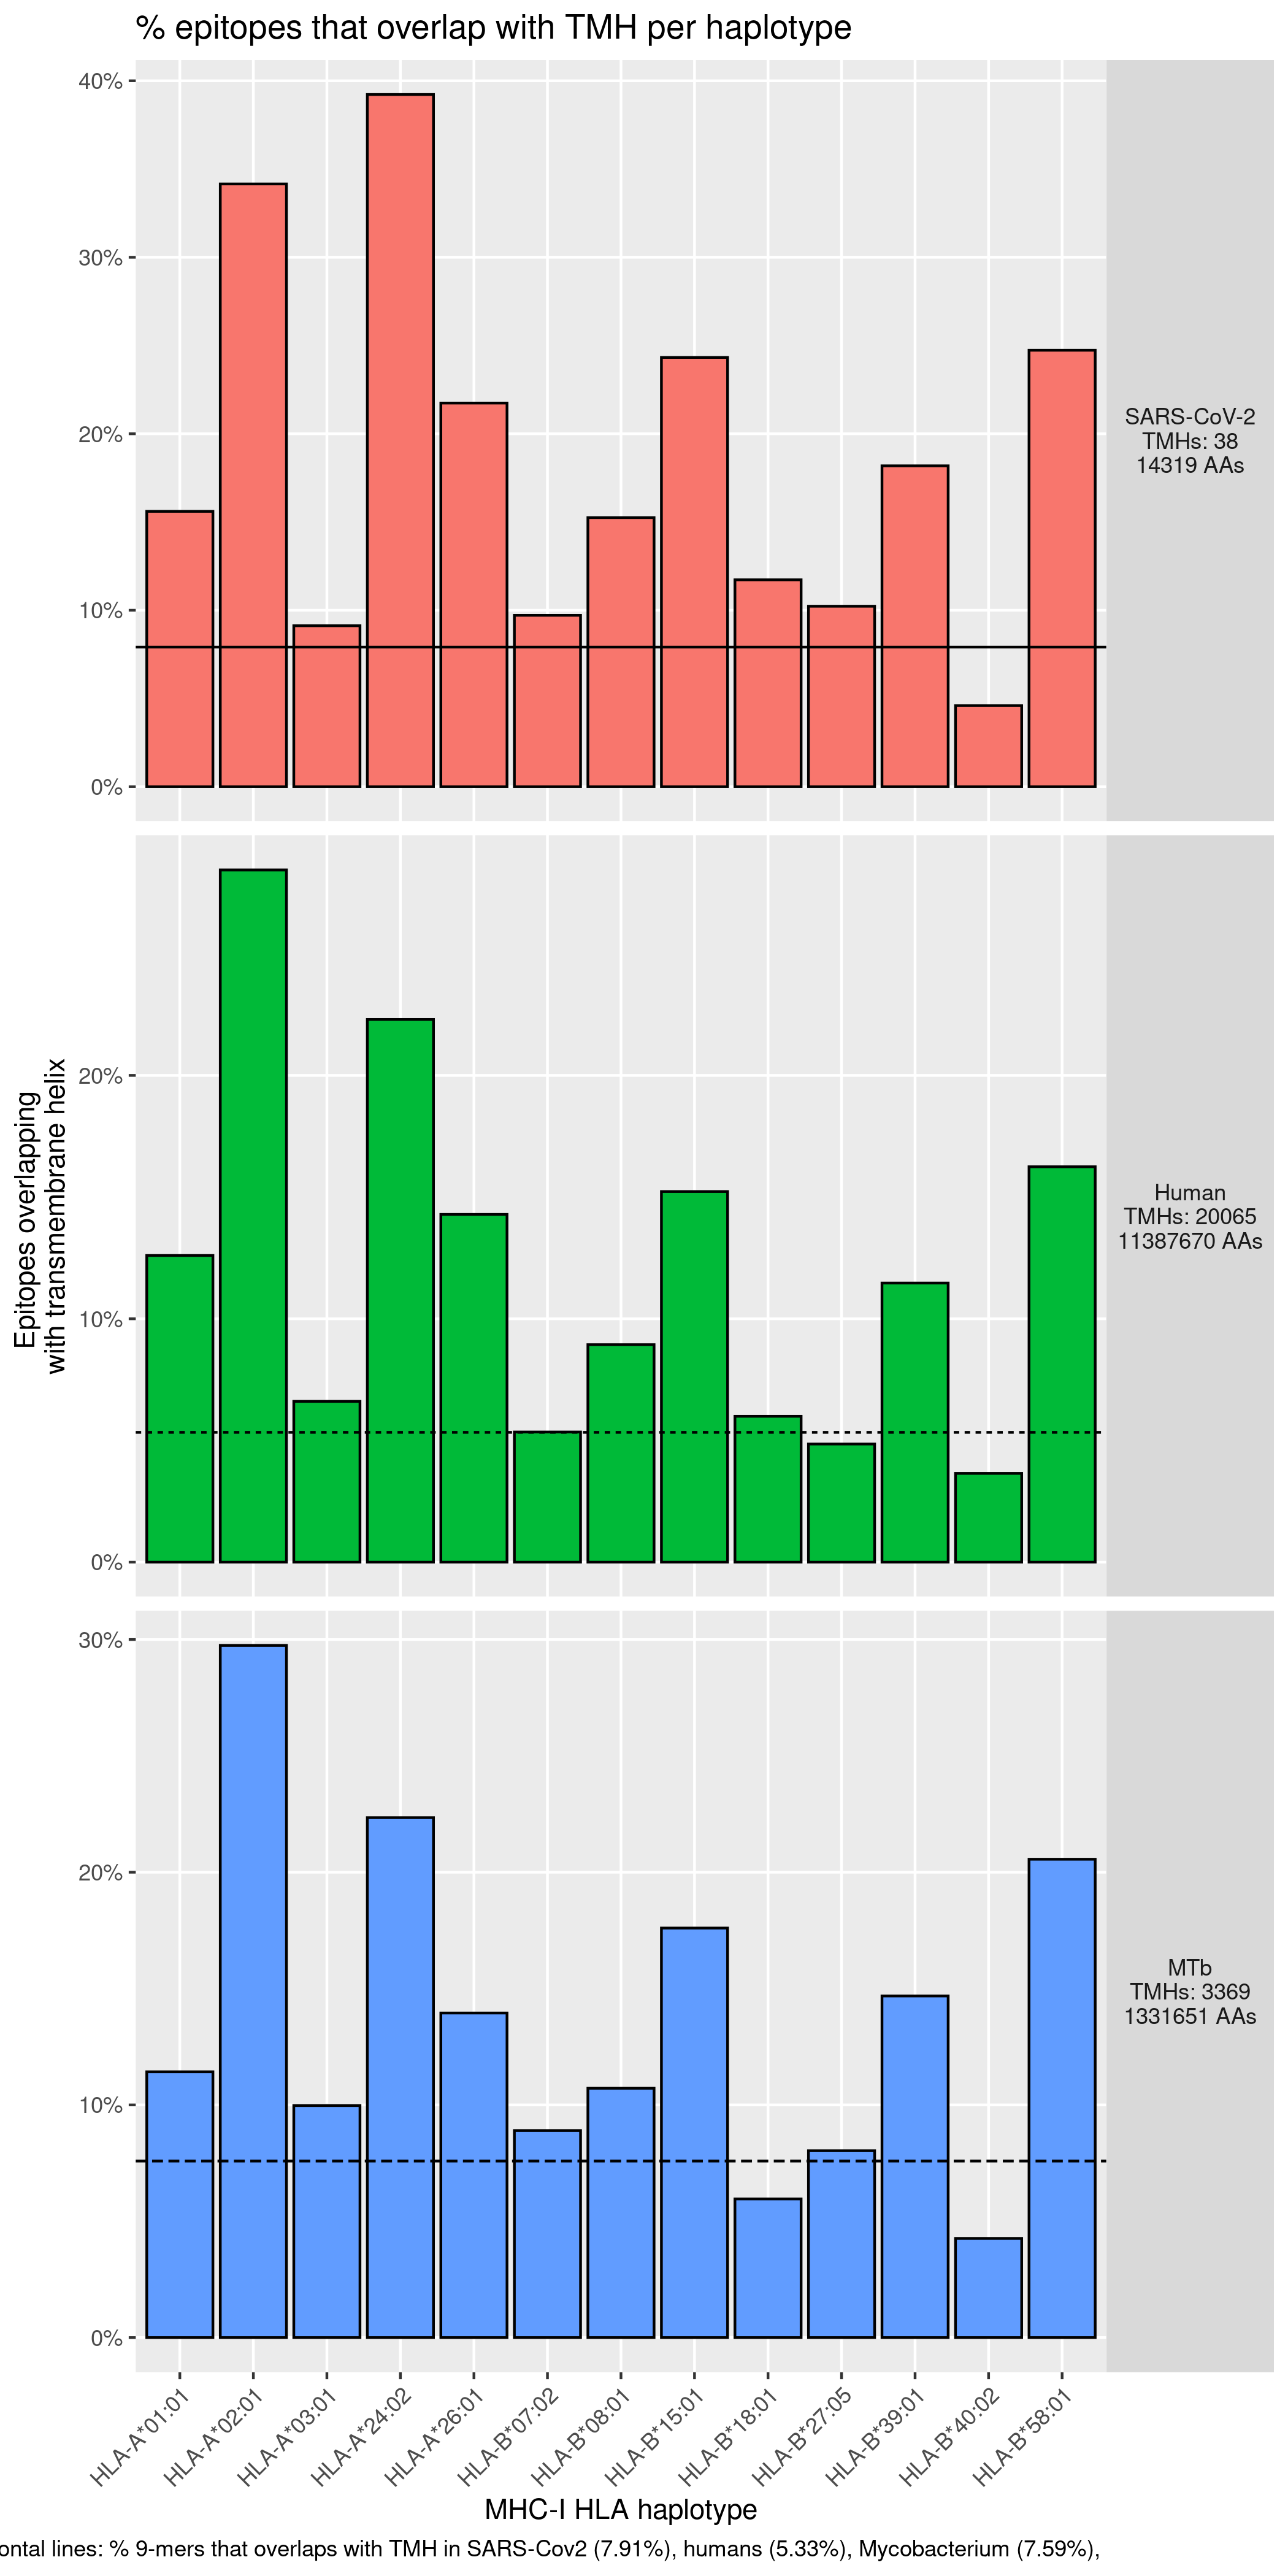
\includegraphics[height=0.9\textheight]{bbbq_1_smart_results/fig_f_tmh_mhc1_2_grid.png}
  \caption{
    Percentage of MHC-I epitopes overlapping with TMHs
    for a human, viral and bacterial proteome.
    The horizontal lines indicate the percentage as expected by chance.
    See table \ref{tab:tmh_binders_mhc1} for the exact TMH and epitope counts.
  }
  \label{fig:1}
\end{figure}

%%%%%%%%%%%%%%%%%%%%%%%%%%%%%%%%%%%%%%%%%%%%%%%%%%%%%%%%%%%%%%%%%%%%%%%%%%%%%%%%
\subsection{MHC-II}
%%%%%%%%%%%%%%%%%%%%%%%%%%%%%%%%%%%%%%%%%%%%%%%%%%%%%%%%%%%%%%%%%%%%%%%%%%%%%%%%

\richel{GvdB: Again a rationale}
Figure \ref{fig:2} shows the percentages of MHC-II epitopes overlapping 
with TMHs for our human, viral and bacterial proteome.
See the supplementary materials (table \ref{tab:tmh_binders_mhc2}) 
for the TMH and epitope counts.
\richel{GvdB: And a conclusion}

\begin{figure}[!htbp]
  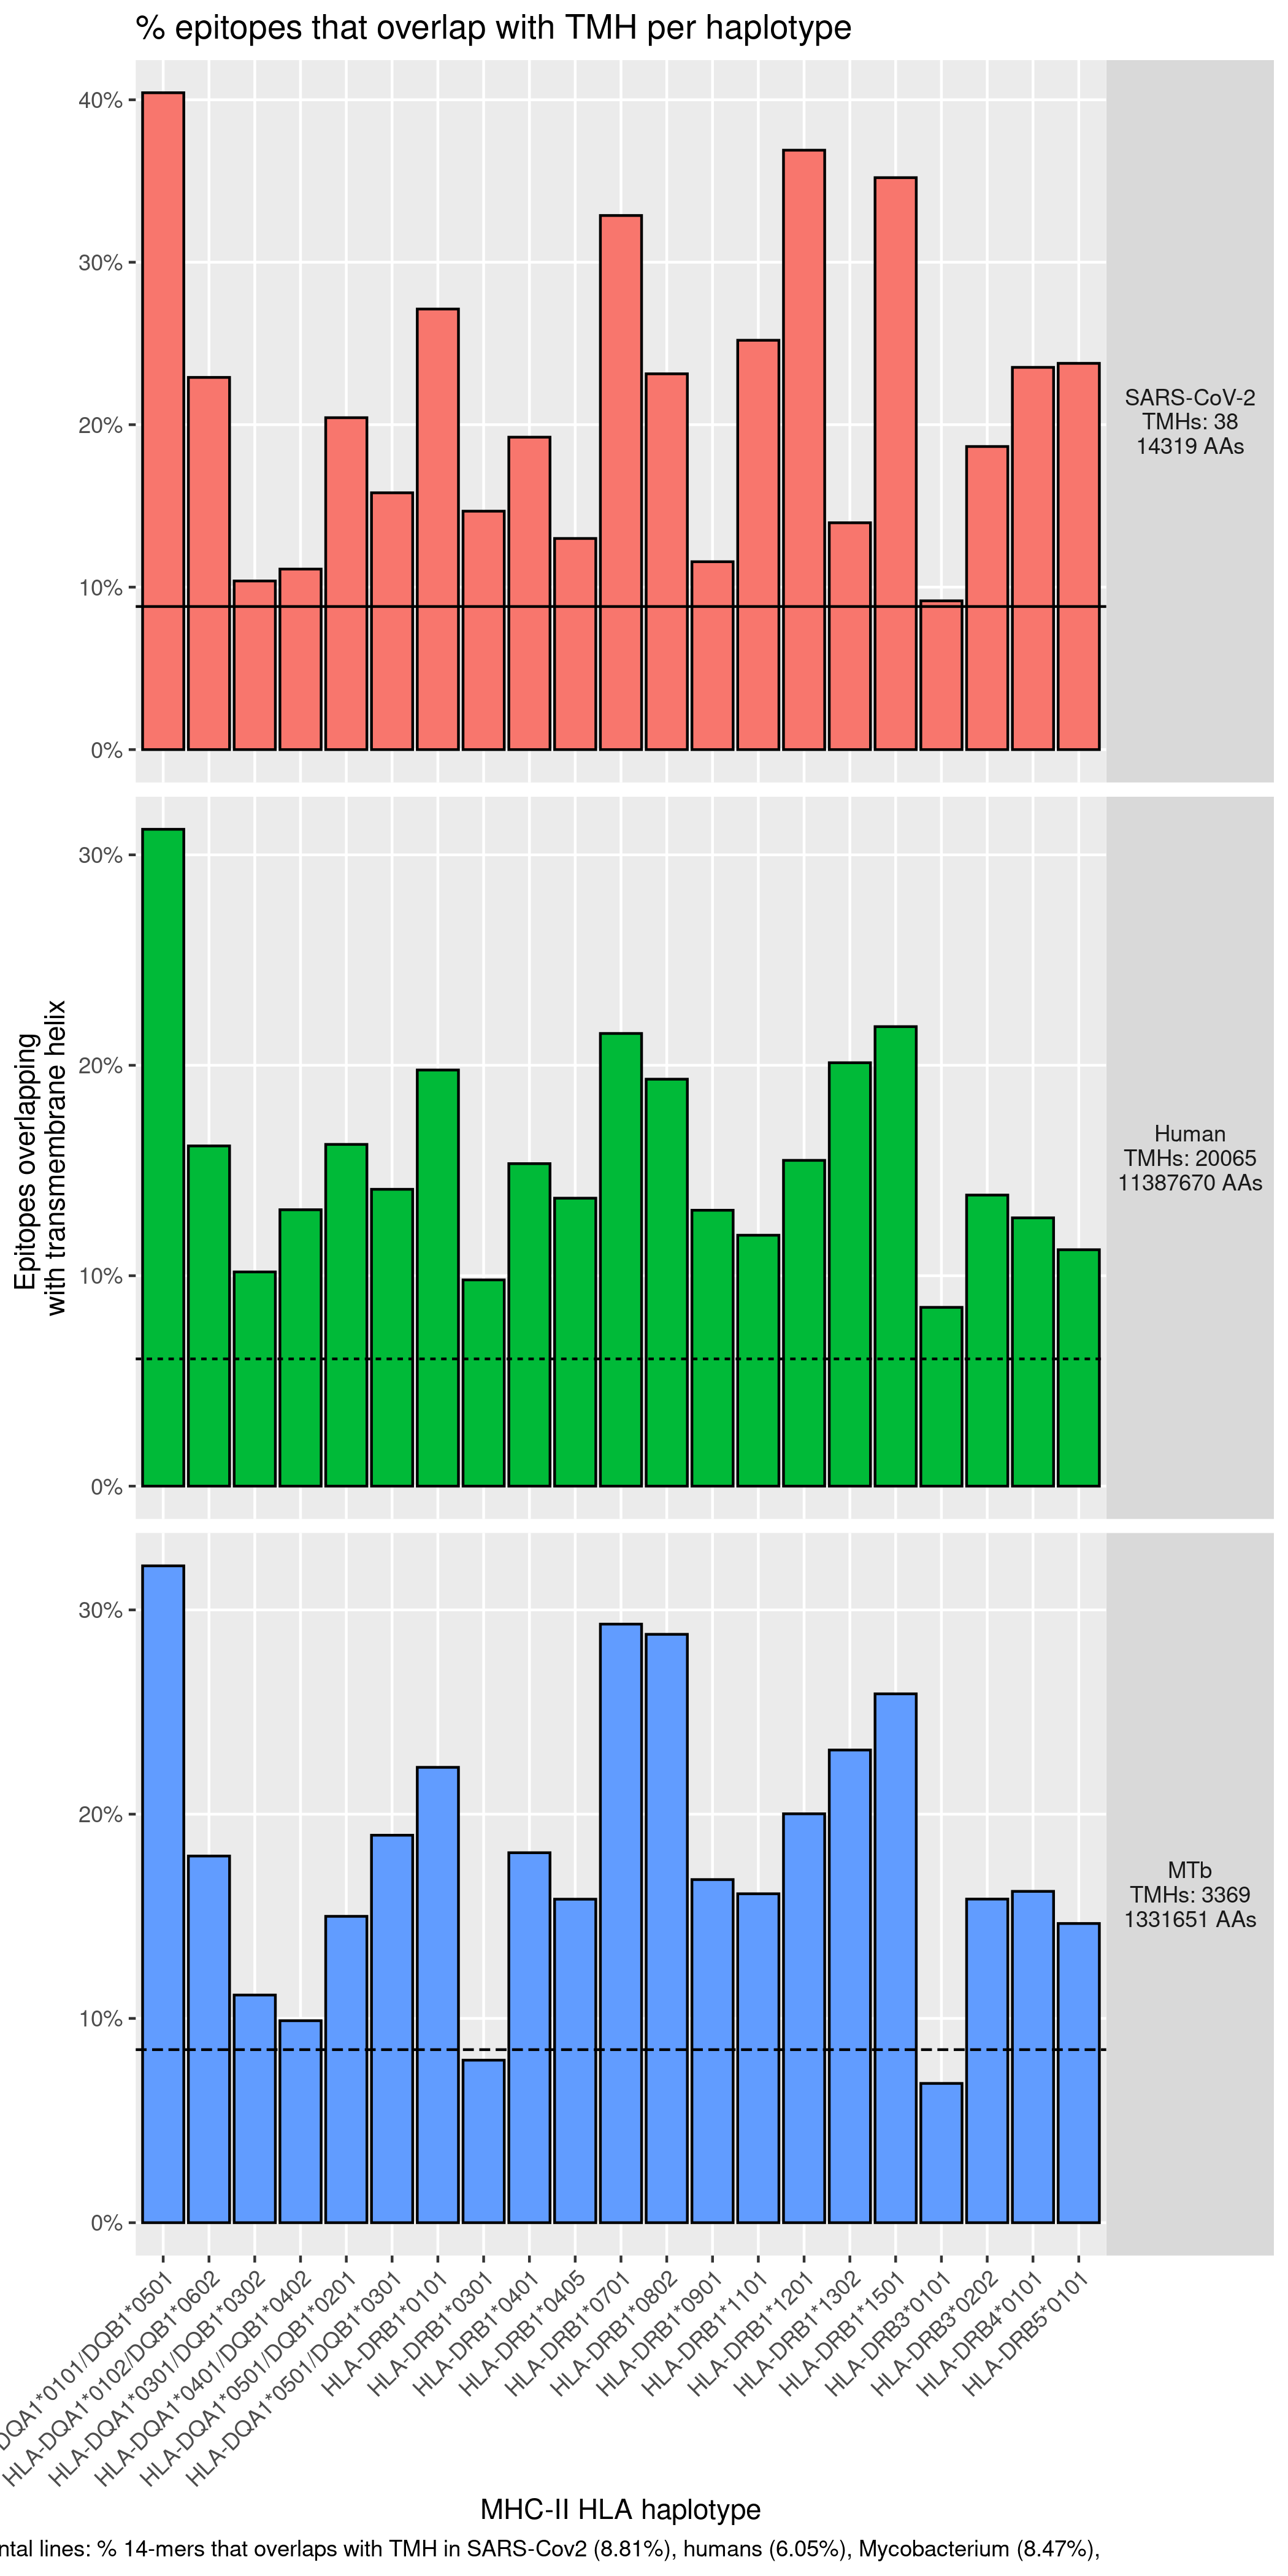
\includegraphics[height=0.9\textheight]{bbbq_1_smart_results/fig_f_tmh_mhc2_2_grid.png}
  \caption{
    Percentage of MHC-II epitopes overlapping with TMHs
    for a human, viral and bacterial proteome.
    The horizontal lines indicate the percentage as expected by chance.
    See table \ref{tab:tmh_binders_mhc2} for the exact TMH and epitope counts.
    Note that for smaller proteomes a percentage of zero is likelier.
  }
  \label{fig:2}
\end{figure}

%%%%%%%%%%%%%%%%%%%%%%%%%%%%%%%%%%%%%%%%%%%%%%%%%%%%%%%%%%%%%%%%%%%%%%%%%%%%%%%%
\subsection{Evolutionary conservation}
%%%%%%%%%%%%%%%%%%%%%%%%%%%%%%%%%%%%%%%%%%%%%%%%%%%%%%%%%%%%%%%%%%%%%%%%%%%%%%%%

\begin{figure}[!htbp]
  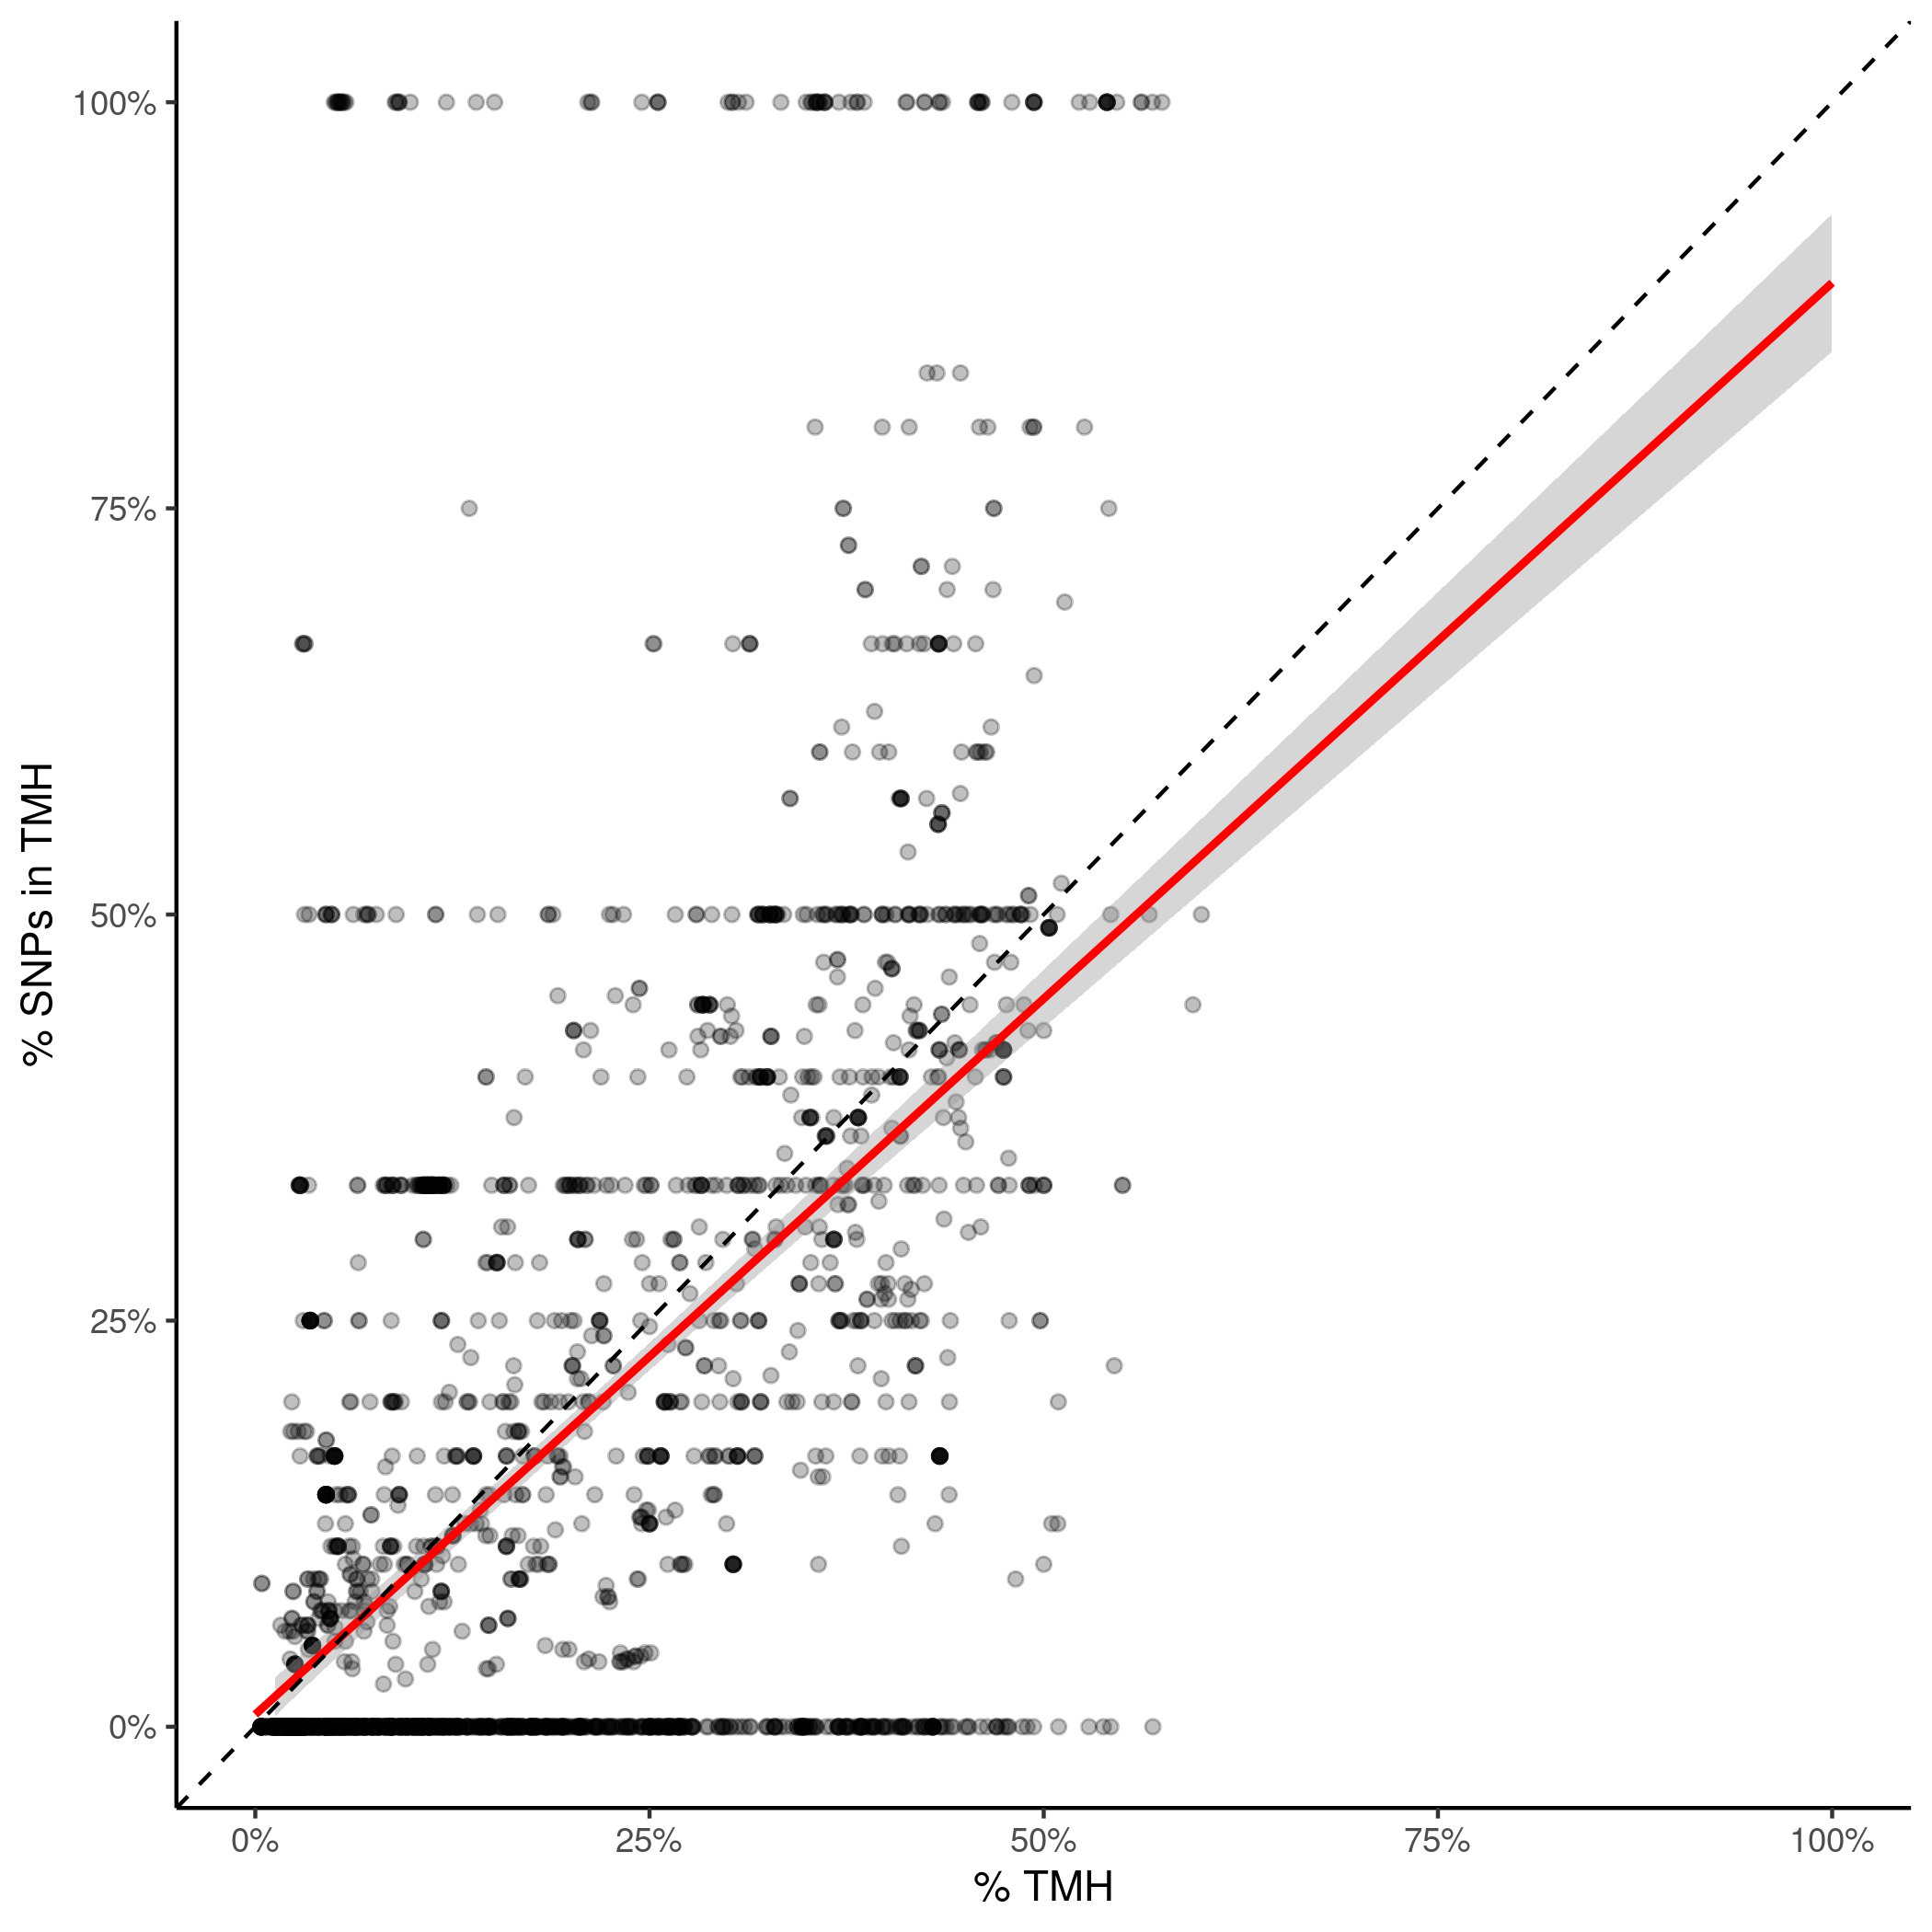
\includegraphics[width=\textwidth]{ncbi_peregrine_results/fig_f_snps_found_and_expected.png}
  \caption{
    Percentage of SNPs found in TMHs.
    Each point resembles one protein, with a predicted percentage of
    TMH (x-axis) and an observed occurrence of SNPs being located
    within a TMH (y-axis).
    The dashed diagonal line shows the expected linear trend line
    if TMHs and soluble protein regions are equally conserved.
    The red line is a linear trend line that includes the membrane-associated
    proteins at the origin. 
    The blue line is a linear trend line that includes only the
    transmembrane proteins.
  }
  \label{fig:f_snps_found_and_expected}
\end{figure}

In the final set of experiments, we addressed the question whether TMHs would be more evolutionary conserved than soluble proteins regions by comparing the occurrences of SNPs in the genome coding for TMHs and soluble protein regions. 
We obtained 1,129 gene names associated with the phrase 'membrane protein'.
These genes are linked to 5,203 proteins
\richel{GvdB: Why so many? Isoforms?}, of which 2,754
are predicted to be transmembrane proteins.
We obtained 4,811 SNPs that resulted in an
amino acids substitution, of which 2,568 were located 
in predicted transmembrane proteins.
Per protein, we predicted the percentages of the gene coding for TMHs and soluble regions
and calculated the percentage of amino acids substitutions
occurring in TMHs.
Per protein, this percentage was plotted as a function of the percentage TMH in figure
\ref{fig:f_snps_found_and_expected}.
We performed a linear regression analysis on the data, with and without
membrane-associated proteins \richel{GvdB: explain clearer}, and calculated the 95\%
confidence interval.
Since the regression curve clearly deviated from the line of equality,
which would be expected if SNPs occur just as likely within transmembrane and soluble protein domains,
this suggests that variations occur more often in soluble 
than in transmembrane protein regions.

To test whether SNPs occur just as likely in soluble as
in transmembrane protein domains, we used a Poisson binomial
distribution. We first calculated the expected number of SNPs
found in TMHs, which is 61,457 SNPs \richel{GvdB: I don’t completely follow this. Based on what?} and multiplied this number by 6.8\% 
of all proteins being a TMH, resulting in the null hypothesis
of 4203 SNPs occurring in TMHs. 
Note that including or excluding
the membrane associated proteins 
has no effect on this statistical test, as the chance 
of a successful trial is zero (there is zero chance
to find a SNP in TMHs if there are none) \richel{GvdB: Also too complex for biologists. Explain in bit more words}.
The actually number of SNPs found in TMHs
was 3889, which is lower than the null hypothesis. 
The chance to find, within TMHs, this amount or less SNPs 
equals $1.6201 \cdot 10^{-9}$.
Using a alpha value of $0.05$, as is common practice for an uninformed
expectation, we conclude that there are significantly less SNPs
in TMHs as expected by chance.
The effect size is that per 1 SNP found in soluble protein
domains, one finds 0.925 SNPs in TMHs.

\begin{figure}[!htbp]
  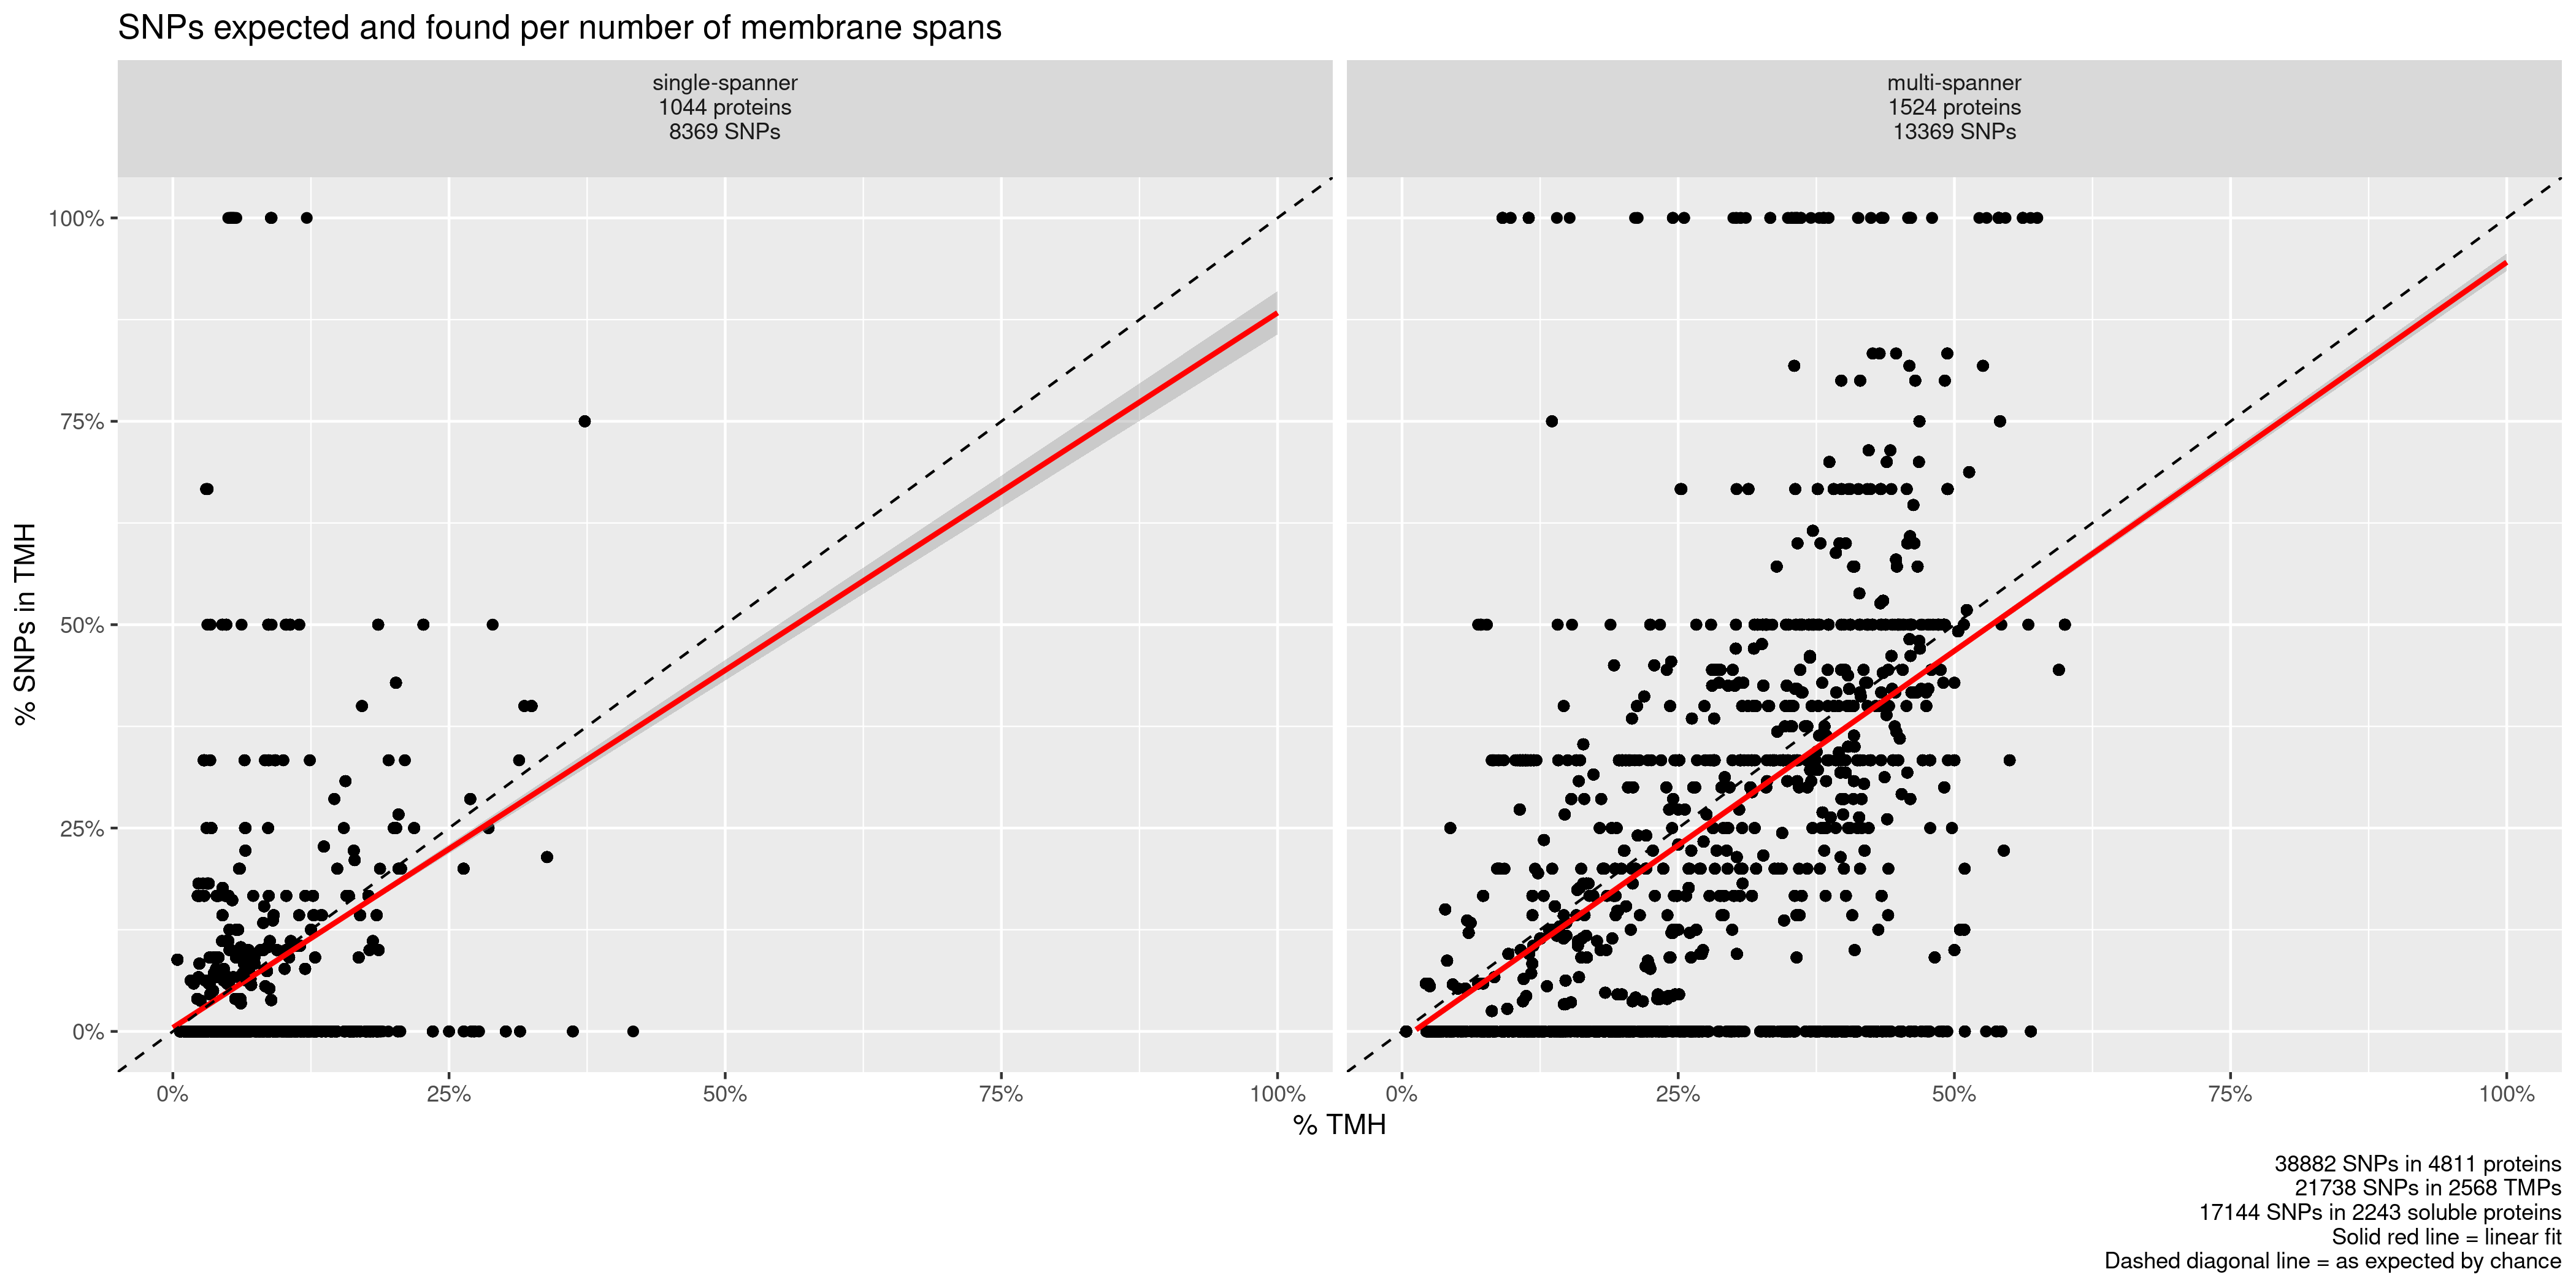
\includegraphics[width=\textwidth]{ncbi_peregrine_results/fig_f_snps_found_and_expected_per_spanner.png}
  \caption{
    Percentage of SNPs found in TMHs per spanner.
    The dashed diagonal lines show the expected linear trend line
    if TMHs and soluble protein regions are equally conserved.
  }
  \label{fig:f_snps_found_and_expected_per_spanner}
\end{figure}
)

We decided to split this analysis based on the number of TMHs
a protein has \richel{Why? Provide brief rationale again. Thus TMH-TMH interactions or something}. We hypothesize that single-spanners (i.e. proteins
with one TMH predicted) are less conserved, when compared to multi-spanners,
as single spanners just need to span a membrane, while multi-spanners
might have interactions between their TMHs, 
for example to accommodate active sites, and 
thus might have additional structural constraints.
As can be seen in figure \ref{fig:f_snps_found_and_expected_per_spanner}, 
both single- and multi-spanners are evolutionarily conserved.

%%%%%%%%%%%%%%%%%%%%%%%%%%%%%%%%%%%%%%%%%%%%%%%%%%%%%%%%%%%%%%%%%%%%%%%%%%%%%%%%
\section{Conclusion}
%%%%%%%%%%%%%%%%%%%%%%%%%%%%%%%%%%%%%%%%%%%%%%%%%%%%%%%%%%%%%%%%%%%%%%%%%%%%%%%%

% \paragraph{General pattern in epitope presentation}

From this study, two important conclusions can be drawn. 
First, the MHC over-presentation of TMHs is likely a general feature 
and predicted to occur for most haplotypes of both MHC-I and -II 
and for humans as well as bacterial and viral pathogens. 
Second, TMHs are more evolutionary conserved that soluble protein motifs, 
at least in the human proteome. 

% \paragraph{Interesting haplotype for SARS-CoV-2}

It is known that an individual's haplotype
influences the dynamics of a pathogen (see,
for example, \cite{eccleston2017host} for HIV) \richel{GvdB: Too vague. How?}.
The bioinformatics pipeline developed in this
study may be interesting to make in silico
predictions of a SARS-CoV-2 infection.
The most prominent example is the (MHC-I)
haplotype HLA-A*24:02,
which is predicted to present four times as much epitopes derived 
from SARS-CoV-2 TMHs than expected by chance.
This may help the immune system to detect a SARS-CoV-2 infection earlier,
and change the infection's dynamics.

%%%%%%%%%%%%%%%%%%%%%%%%%%%%%%%%%%%%%%%%%%%%%%%%%%%%%%%%%%%%%%%%%%%%%%%%%%%%%%%%
\section{Discussion}
%%%%%%%%%%%%%%%%%%%%%%%%%%%%%%%%%%%%%%%%%%%%%%%%%%%%%%%%%%%%%%%%%%%%%%%%%%%%%%%%

\richel{
  GvdB:

  Discussion section needs some work, 
  as here interpretation of the results needs to be given. 
  What is the consequence of the findings? Why is it important. 

  Now it is just a list of potential reasons why the results might be flawed. 
  While this is in principle OK, 
  it is also nitpicking as some things affect only a limited number of 
  proteins (like selenoproteins) 
  or you’d expect changes in the other direction (wrong prediction of TMHs for bacteria). 

  So offer interpretations. 
  The second part of the introduction would fit here well. I can also help with this.
}

% RJCB: moved this from Introduction to Discussion.
%
% \paragraph{Does MHC-I present TMH-derived epitopes from pathogens as often?}
% 
% It is important that MHC-I presents both the peptides of the 
% (healthy) cell, as well as possible pathogen-derived peptides when the
% cell is infected. As described above, MHC-I presents TMH-derived epitopes 
% from the human host more often. It is unknown if MHC-I has the same
% dedication to present epitopes that stem from TMHs derived from
% proteins produced by pathogen, either would the pathogen
% be a virus or 
% a bacterium.
% 
% \paragraph{MHC-II is expected to present TMHs}
% 
% If presentation of TMHs on MHC-I would bring an evolutionary advantage 
% in the recognition of pathogens by the immune system, 
% it would follow that this is equally important for MHC-II, 
% especially as the help of CD4+ T cells is needed for a long lasting CD8+ T cell 
% response (\cite{novy2007cd4}). 
% The mechanism to detect foreign TMHs by MHC-II would be unknown, 
% similar to the discovery that MHC-I presents TMHs.
% 
% \paragraph{Does MHC-II present TMH-derived epitopes from pathogens as often?}
% 
% It is unknown if MHC-II, like MHC-I, 
% presents TMH-derived epitopes as often, either 
% in humans,
% bacteria or viruses.
% 
% \paragraph{Selection undetectable in whole proteome}
% 
% In general, on would hope that evolutionary selection results in
% an immune system that as most attentive for loci that are
% essential for a virus, as these will be most conserved.
% In SARS-CoV-2, for example, there is preliminary evidence that the strongest
% selection pressure is upon residues that changes its 
% virulence (\cite{velazquez2020positive}).
% These loci, however, only account for a small part of a pathogen's proteome.
% Additionally, these essential parts differ widely between pathogens.
% Because of this scarcity and variance in targets, 
% one can imagine that the human immune system 
% is not tailored to detect these sites, 
% as hinted by upon by the aforementioned influenza study.
% 
% \paragraph{Selection may be detectable in TMHs}
% 
% TMHs, on the other hand, also have their function constraints, 
% yet can occur multiple time a pathogen's proteome.
% One can safely assume a pathogen's proteome contains multiple TMHs.
% Therefore, it may be beneficial for the host
% if its immune system would be more attentive towards TMHs.
% And maybe this has already happened: MHC-I already detects hydrophobic
% peptides. This feature, however, may also be caused by selection
% to detect hydrophobic regions in the soluble proteins of pathogens.
% It is unknown, when focusing on TMHs only, if a signal of selection
% can be detected.
% 
% \paragraph{Use of protein data in phylogenetics}
% 
% When using DNA sequences, one can use a skewed rate
% in non- versus synonymous mutation
% to detect the signature of selection (\cite{murrell2015gene}).
% Using AA sequences, however, has its advantages,
% as its is closer to the actual phenotype
% selection acts upon: DNA may never be transcribed to RNA,
% or its RNA may never be translated (\cite{diz2012proteomics}).
% When using a proteome in phylogenetic research,
% we know that the majority of proteins are selected to just
% maintain their function most of the time, where
% is the time spans there is selection, only a few AAs
% can actually increase the 'fitness' of the
% protein (\cite{anisimova2009investigating}).
% There, when generalizing the dynamics of mostly purifying selection (to maintain
% a protein's function) and a short duration of positive selection,
% those genes that are selected cannot be detected (\cite{yang2000statistical}).

\subsection{Elution studies}

% \paragraph{False positives}

We assume that epitopes 
derived from TMHs are actually presented by MHC-I and MHC-II.
Our analysis (at subsection \ref{subsec:elution_studies}) 
finds that 1.4\% (for MHC-I) and 4.0% (for MHC-II) 
of the epitopes presented 
overlap with a TMH.
It is unsure if this a true finding or a false positive.
One source of noise would stem from imperfect predictions
by the topology prediction software used. 
We have counteracted this by using two different topology prediction
software and confirm these have similar results.
Two biological sources of noise \richel{GvdB: What do you mean by noise?}
are defective ribosomal products (DRiPs) (\cite{yewdell1996defective}) 
and peptide fusion \cite{delong2016pathogenic},
two processes that both result in peptide fragments
that did not originate from genome directly.
Note however, that both elution studies have a
methodological bias caused by mass spectronomy,
as hydrophobic fragments are detected less 
by mass spectronomy.

\subsection{\% epitopes overlapping with TMHs}

\subsection{Evolutionary conservation}

\richel{GvdB: This might be relevant, but you need to explain why it is relevant. Thus compare your findings with previous efforts to look at conservation of TMHs}
% \paragraph{synonymous mutations}
%
In our evolutionary experiment, 
we removed variations that were synonymous mutations (i.e.
resulted in the same amino acid, from a different genetic code) 
from our analysis.
There is evidence, however, that these synonymous mutations
do have an effect and may even be evolutionary selected 
for (\cite{hunt2009silent}).
As the possible effect of synonymous mutations is ignored by our
topology prediction software, we do so as well.



% \paragraph{Low number of SNPs}

The NCBI dbSNP database contains millions of SNPs.
As the NCBI API constrains its users to three calls per second,
we had to limited the extent of our analysis.

\richel{GvdB: This can go to the methods or results.}
% \paragraph{Selection of SNPs}
%
We selected to analyze SNPs with the lowest SNP ID first.
This means we have a bias for picking SNPs with
an earlier discovery date.
We expect this bias to be biologically irrelevant
and we find no clear evidence of a bias, as
shown in figure \ref{fig:n_tmhs_per_protein}.
Still, the best way to interpret this figure
is open to discussion.

% We concluded that the
% epitopes that MHC-I presents are [as/not as] likely 
% to be derived from TMH within either a human host and its bacterial pathogen.
% Because a bacterium does not infect a cell, thus its peptides
% will not be presented by MHC-I, this result is [unexpected/expected]
% 
% We aimed our evolutionary experiment at TMHs, because these can
% be predicted well from a protein structure,
% are common structures and are present in all pathogens. 
% We could have done the same experiment on beta-turn,
% as also these can be predicted well (\cite{petersen2010netturnp}),
% are common structures and are present in all pathogens.
% 
% The human immune system and human pathogen are in an evolutionary
% arms race: our immune systems is selected for the detection
% of pathogens, whereas pathogens are selected to avoid detection.
% From a pathogen's point of view, however, this struggle 
% is of only minor importance:
% in seasonal influenza, for example, the selection pressure
% exerted by the immune system was only limited (\cite{han2019individual}).

%%%%%%%%%%%%%%%%%%%%%%%%%%%%%%%%%%%%%%%%%%%%%%%%%%%%%%%%%%%%%%%%%%%%%%%%%%%%%%%%
\section{Acknowledgments}
%%%%%%%%%%%%%%%%%%%%%%%%%%%%%%%%%%%%%%%%%%%%%%%%%%%%%%%%%%%%%%%%%%%%%%%%%%%%%%%%

We thank the Center for Information Technology of the University 
of Groningen for its support and for providing access to the Peregrine 
high performance computing cluster. 
Additionally, we would like to thank Sci-Hub (\cite{himmelstein2018sci})
for allowing us to read paywalled articles while working from home.
\richel{GvdB: Should we include Maxim? He did the alignment of Mycobacterium tuberculosis. Let’s also ask Frans.}

%%%%%%%%%%%%%%%%%%%%%%%%%%%%%%%%%%%%%%%%%%%%%%%%%%%%%%%%%%%%%%%%%%%%%%%%%%%%%%%%
\section{Data Accessibility}
%%%%%%%%%%%%%%%%%%%%%%%%%%%%%%%%%%%%%%%%%%%%%%%%%%%%%%%%%%%%%%%%%%%%%%%%%%%%%%%%

All code is archived at \url{http://github.com/richelbilderbeek/someplace},
with DOI \url{https://doi.org/12.3456/zenodo.1234567}.

%%%%%%%%%%%%%%%%%%%%%%%%%%%%%%%%%%%%%%%%%%%%%%%%%%%%%%%%%%%%%%%%%%%%%%%%%%%%%%%%
\section{Authors' contributions}
%%%%%%%%%%%%%%%%%%%%%%%%%%%%%%%%%%%%%%%%%%%%%%%%%%%%%%%%%%%%%%%%%%%%%%%%%%%%%%%%

RJCB and FB conceived the idea for this research. 
RJCB wrote the code.
RJCB and FB wrote the article.

%%%%%%%%%%%%%%%%%%%%%%%%%%%%%%%%%%%%%%%%%%%%%%%%%%%%%%%%%%%%%%%%%%%%%%%%%%%%%%%%
% Bibliography
%%%%%%%%%%%%%%%%%%%%%%%%%%%%%%%%%%%%%%%%%%%%%%%%%%%%%%%%%%%%%%%%%%%%%%%%%%%%%%%%
% MEE style
\bibliographystyle{mee}
\bibliography{bbbq_article}
%%%%%%%%%%%%%%%%%%%%%%%%%%%%%%%%%%%%%%%%%%%%%%%%%%%%%%%%%%%%%%%%%%%%%%%%%%%%%%%%


%%%%%%%%%%%%%%%%%%%%%%%%%%%%%%%%%%%%%%%%%%%%%%%%%%%%%%%%%%%%%%%%%%%%%%%%%%%%%%%%
\appendix
\section{Supplementary materials}
%%%%%%%%%%%%%%%%%%%%%%%%%%%%%%%%%%%%%%%%%%%%%%%%%%%%%%%%%%%%%%%%%%%%%%%%%%%%%%%%

%%%%%%%%%%%%%%%%%%%%%%%%%%%%%%%%%%%%%%%%%%%%%%%%%%%%%%%%%%%%%%%%%%%%%%%%%%%%%%%%
\subsection{Differences with Bianchi et al., 2017}
%%%%%%%%%%%%%%%%%%%%%%%%%%%%%%%%%%%%%%%%%%%%%%%%%%%%%%%%%%%%%%%%%%%%%%%%%%%%%%%%

A part of this study does the same analysis as Bianchi et al., 2017.
Here we describe the deviations, which are about the use of different
software and the use of a different definition of what a binder is.

% Percentage of spots and spots that overlap with a TMH
\input{bbbq_1_smart_results/table_f_tmh_2.latex}

% \paragraph{IC50 prediction software}

The earlier study uses \verb;epitope-prediction; a hand-crafted method, 
that has been trained on MHC-I haplotypes only,
which is used here again. For MHC-II IC50 predictions, the
'mhcnuggetsr' R package is used.

% \paragraph{Definition of what a binder is}

The earlier study defines a peptide a binder (for a haplotype), 
if \emp{within the peptide} in which it is found, 
is within the peptides with the 2\% lowest IC50 values.
This can be seen at \url{https://github.com/richelbilderbeek/bianchi_et_al_2017/blob/master/predict-binders.R},
where the binders are written to file.

In this study, a peptide is defined a binder (for a haplotype), 
if within a \emp{proteome} in which it is found, 
is within the peptides with the 2\% lowest IC50 values,
where our previous study used the lowest 2\% IC50 values
within each \emp{protein}.
Subsection \ref{subsec:ic50s_per_haplotype} shows the IC50 values
for a binder per haplotype.

% \paragraph{Selenoproteins}

Our previous study used the TMHMM web server
to predict TMHs.
The desktop version of TMHMM, however, gives an
error message on the 25 selenoproteins found in the human
reference proteome.
For the sake of reproducible research, we use the desktop version (as
we can call it from scripts) and, due to this, we removed the
selenoproteins from this analysis.

%%%%%%%%%%%%%%%%%%%%%%%%%%%%%%%%%%%%%%%%%%%%%%%%%%%%%%%%%%%%%%%%%%%%%%%%%%%%%%%%
\subsection{Minor methods}
%%%%%%%%%%%%%%%%%%%%%%%%%%%%%%%%%%%%%%%%%%%%%%%%%%%%%%%%%%%%%%%%%%%%%%%%%%%%%%%%

PureseqTM does not predict the topology
of proteins that have less than three amino acids. 
The TRDD1 ('T cell receptor delta diversity 1') protein,
however, is two peptides long. 
The R package \verb;pureseqtmr;, however, 
predicts that mono- and di-peptides are cytosolic.

%%%%%%%%%%%%%%%%%%%%%%%%%%%%%%%%%%%%%%%%%%%%%%%%%%%%%%%%%%%%%%%%%%%%%%%%%%%%%%%%
\subsection{Minor discussion}
%%%%%%%%%%%%%%%%%%%%%%%%%%%%%%%%%%%%%%%%%%%%%%%%%%%%%%%%%%%%%%%%%%%%%%%%%%%%%%%%

% \paragraph{Bacteria have a different cell membrane}

In this experiment we predicted epitopes that overlap with 
TMHs from a human, bacterial and viral proteome,
would these proteins be expressed in a human host.
Bacteria, however have different cell membranes and cell walls, 
hence different structural requirements for a TMH.
Both topology prediction tools were trained to recognize
human TMHs, thus we cannot be sure that
the transmembrane regions predicted in bacterial proteins
are actually part of an integral membrane protein.
For the purpose of this study, we assume the 
error in topology predictions to be unbiased way towards topology.
In other words: that a bacterial TMH is incorrectly
predicted to be absent just as often as it is incorrectly
predicted to be present elsewhere.

% \paragraph{False positives in SNPs}

Regarding the evolutionary conservation of TMHs using SNPs,
again, it is estimated that approximately ten percent
of SNPs is a false positive that result from the methods to determine
a SNP. One example is that sequence variations are incorrectly
detected due to highly similar duplicated sequences \cite{musumeci2010single}.
We assume that these duplications occur as often in TMHs as in
regions around these, hence we expect this not to affect our results.

%%%%%%%%%%%%%%%%%%%%%%%%%%%%%%%%%%%%%%%%%%%%%%%%%%%%%%%%%%%%%%%%%%%%%%%%%%%%%%%%
\subsection{IC50s per haplotype}
\label{subsec:ic50s_per_haplotype}
%%%%%%%%%%%%%%%%%%%%%%%%%%%%%%%%%%%%%%%%%%%%%%%%%%%%%%%%%%%%%%%%%%%%%%%%%%%%%%%%

Per target proteome (i.e. human, SARS-CoV-2, Mycobacterium tuberculosis),
we collected all 9-mers (for MHC-I) and 14-mers (for MHC-II),
after removing the selenoproteins and proteins that are shorter
than the epitope length.
From these epitopes, per MHC haplotype,
we predicted the IC50 (in nM) using \verb;epitope-prediction; (for MHC-I)
and MHCnuggets (for MHC-II). 
Here, we show the IC50 value per haplotype that
is used to determine if a peptide binds to the haplotype's MHC
for MHC-I (see table \ref{tab:ic50_binders_mhc1}) and 
MHC-II (see table \ref{tab:ic50_binders_mhc2}).

% tab:ic50_binders_mhc1
\input{bbbq_1_smart_results/table_ic50_binders_mhc1_2.latex}

% tab:ic50_binders_mhc2
\input{bbbq_1_smart_results/table_ic50_binders_mhc2_2.latex}

%%%%%%%%%%%%%%%%%%%%%%%%%%%%%%%%%%%%%%%%%%%%%%%%%%%%%%%%%%%%%%%%%%%%%%%%%%%%%%%%
\subsection{MHC-I}
%%%%%%%%%%%%%%%%%%%%%%%%%%%%%%%%%%%%%%%%%%%%%%%%%%%%%%%%%%%%%%%%%%%%%%%%%%%%%%%%

\begin{figure}[!htbp]
  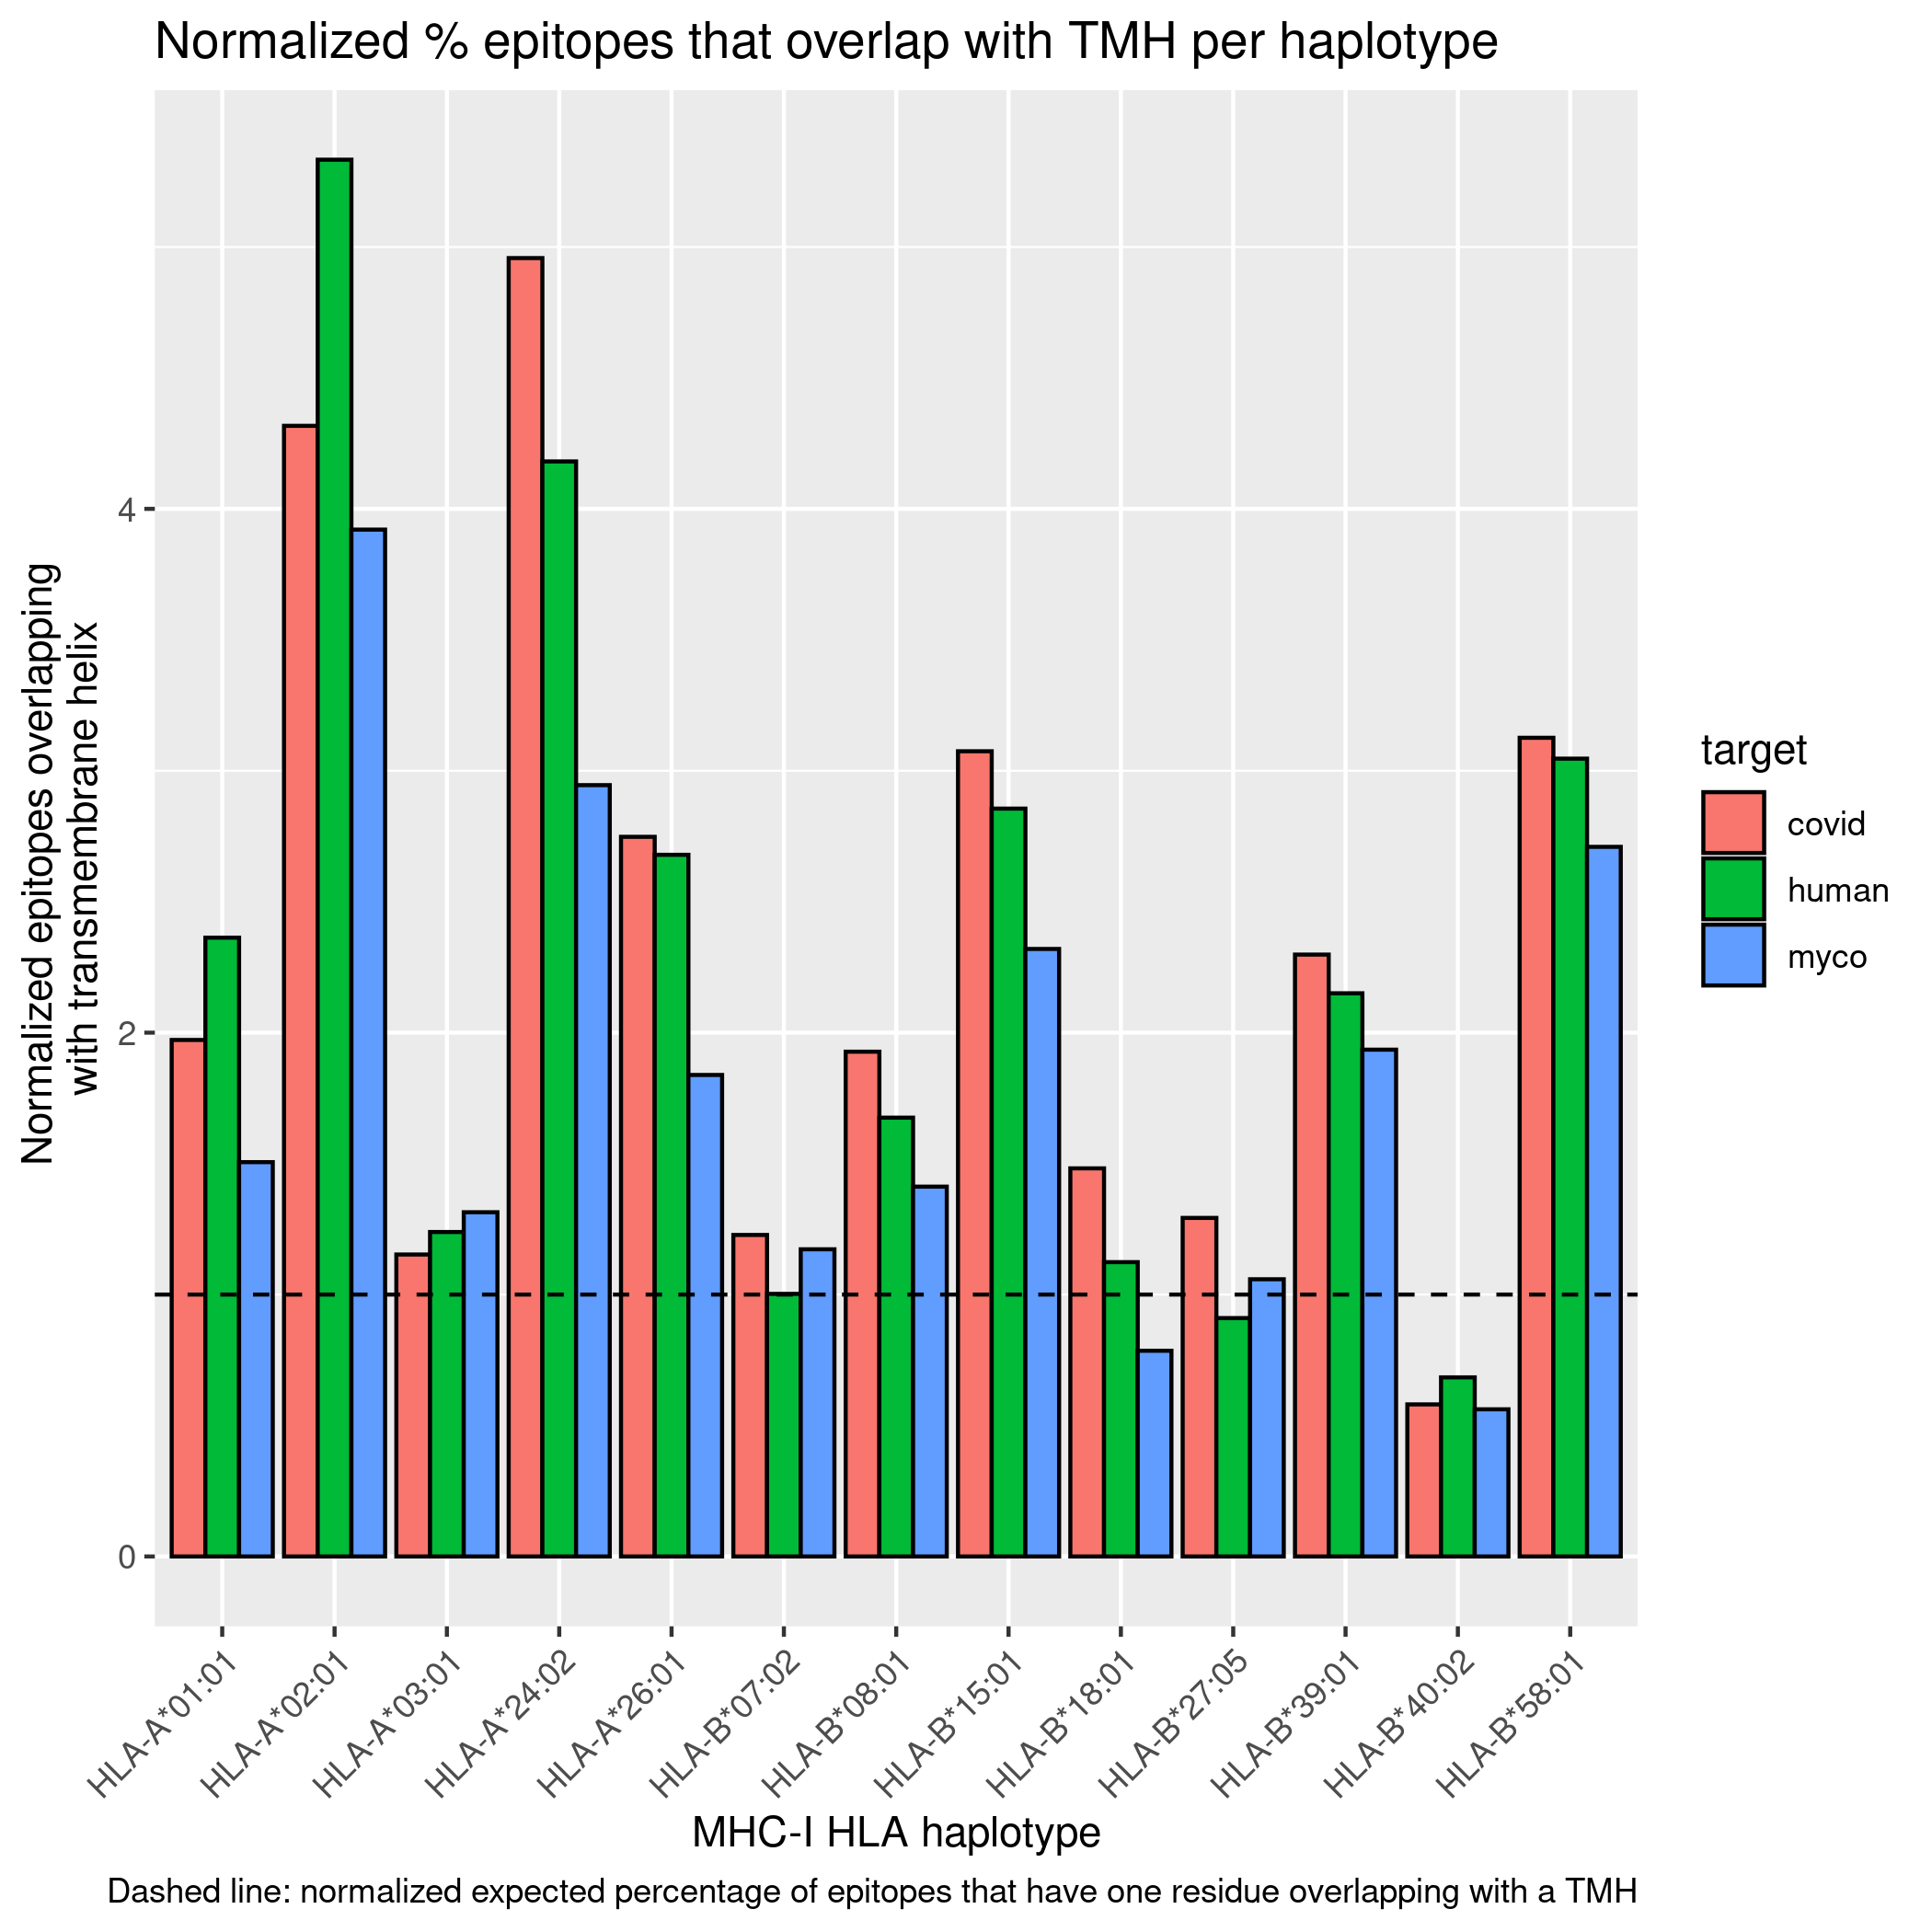
\includegraphics[width=\textwidth]{bbbq_1_smart_results/fig_f_tmh_mhc1_2_normalized.png}
  \caption{
    Normalized proportion of MHC-I epitopes overlapping with TMHs
    for human, viral and bacterial proteomes.
    Legend: covid = SARS-CoV-2,
    human = homo sapiens, myco = Mycobacterium tuberculosis
  }
  \label{fig:f_tmh_mhc1_normalized}
\end{figure}

% Label: tab:tmh_binders_mhc1
\input{bbbq_1_smart_results/table_tmh_binders_mhc1_2.latex}

%%%%%%%%%%%%%%%%%%%%%%%%%%%%%%%%%%%%%%%%%%%%%%%%%%%%%%%%%%%%%%%%%%%%%%%%%%%%%%%%
\subsection{MHC-II}
%%%%%%%%%%%%%%%%%%%%%%%%%%%%%%%%%%%%%%%%%%%%%%%%%%%%%%%%%%%%%%%%%%%%%%%%%%%%%%%%

\begin{figure}[!htbp]
  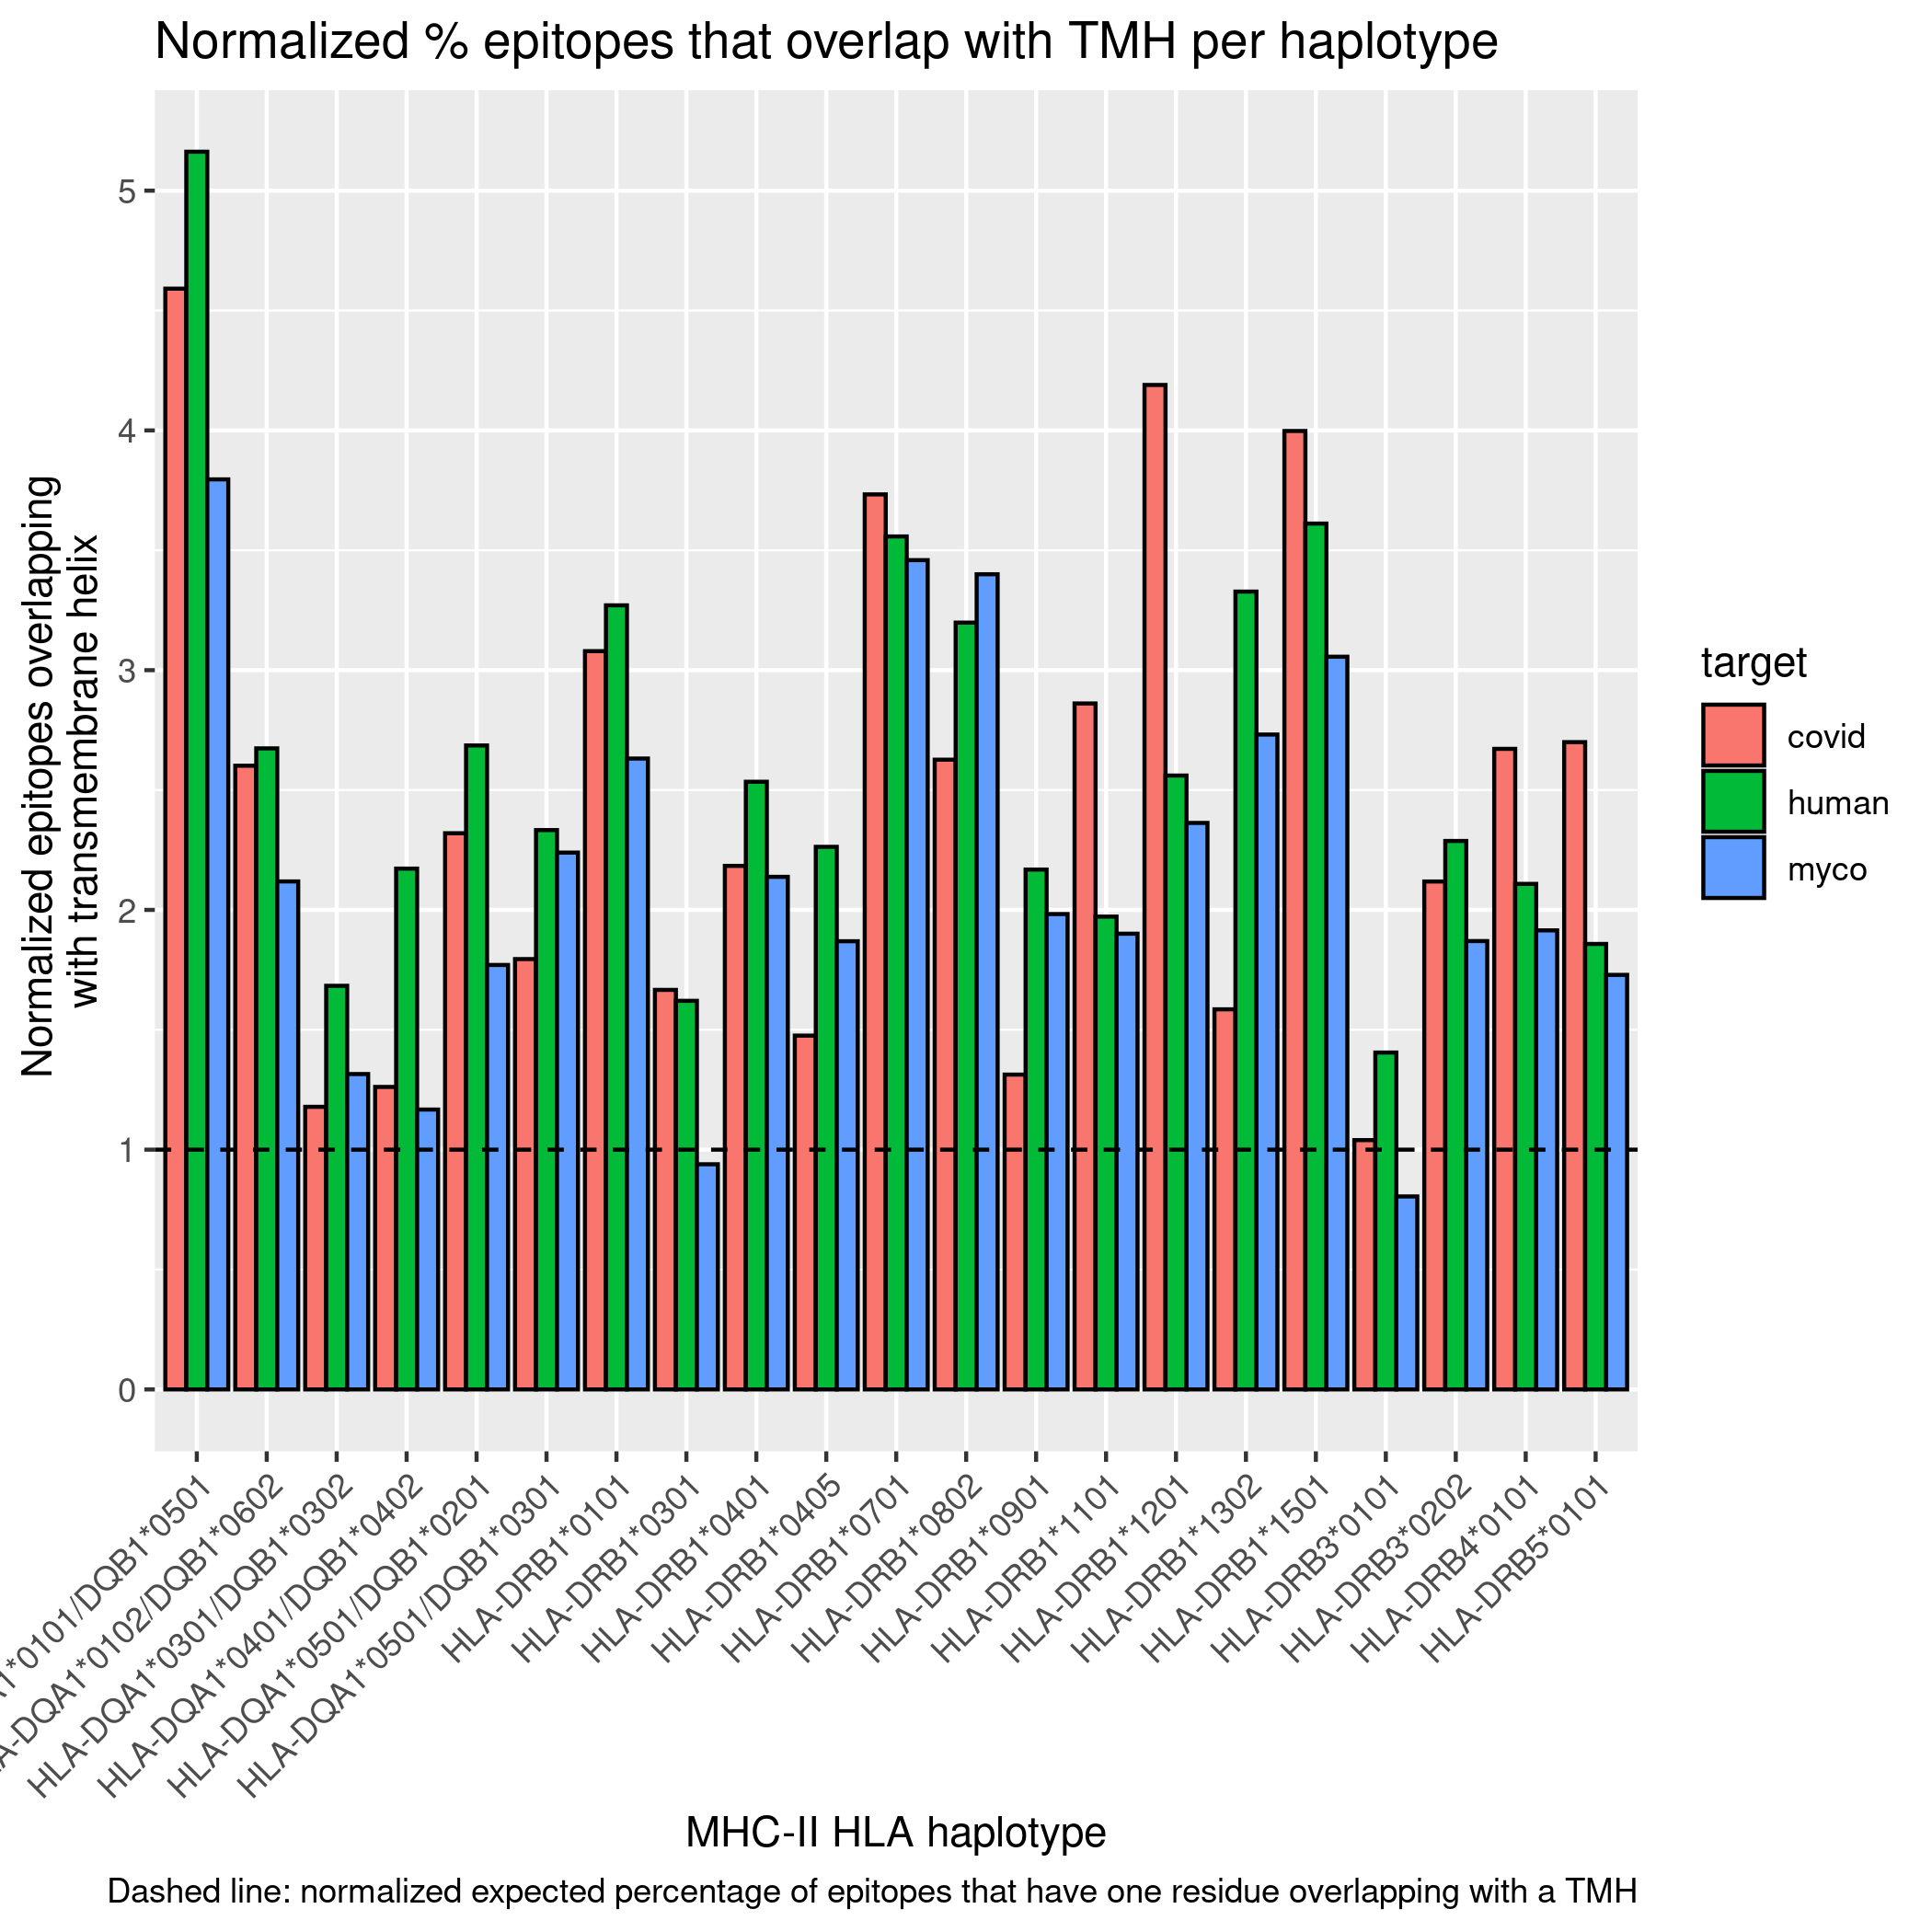
\includegraphics[width=\textwidth]{bbbq_1_smart_results/fig_f_tmh_mhc2_2_normalized.png}
  \caption{
    Normalized proportion of MHC-II epitopes overlapping with TMHs
    for human, viral and bacterial proteomes.
    Legend: covid = SARS-CoV-2,
    human = homo sapiens, myco = Mycobacterium tuberculosis
  }
  \label{fig:f_tmh_mhc2_normalized}
\end{figure}

% Label: tab:tmh_binders_mhc2
\input{bbbq_1_smart_results/table_tmh_binders_mhc2_2.latex}

%%%%%%%%%%%%%%%%%%%%%%%%%%%%%%%%%%%%%%%%%%%%%%%%%%%%%%%%%%%%%%%%%%%%%%%%%%%%%%%%
\subsection{Evolutionary conservation}
%%%%%%%%%%%%%%%%%%%%%%%%%%%%%%%%%%%%%%%%%%%%%%%%%%%%%%%%%%%%%%%%%%%%%%%%%%%%%%%%

\begin{figure}[!htbp]
  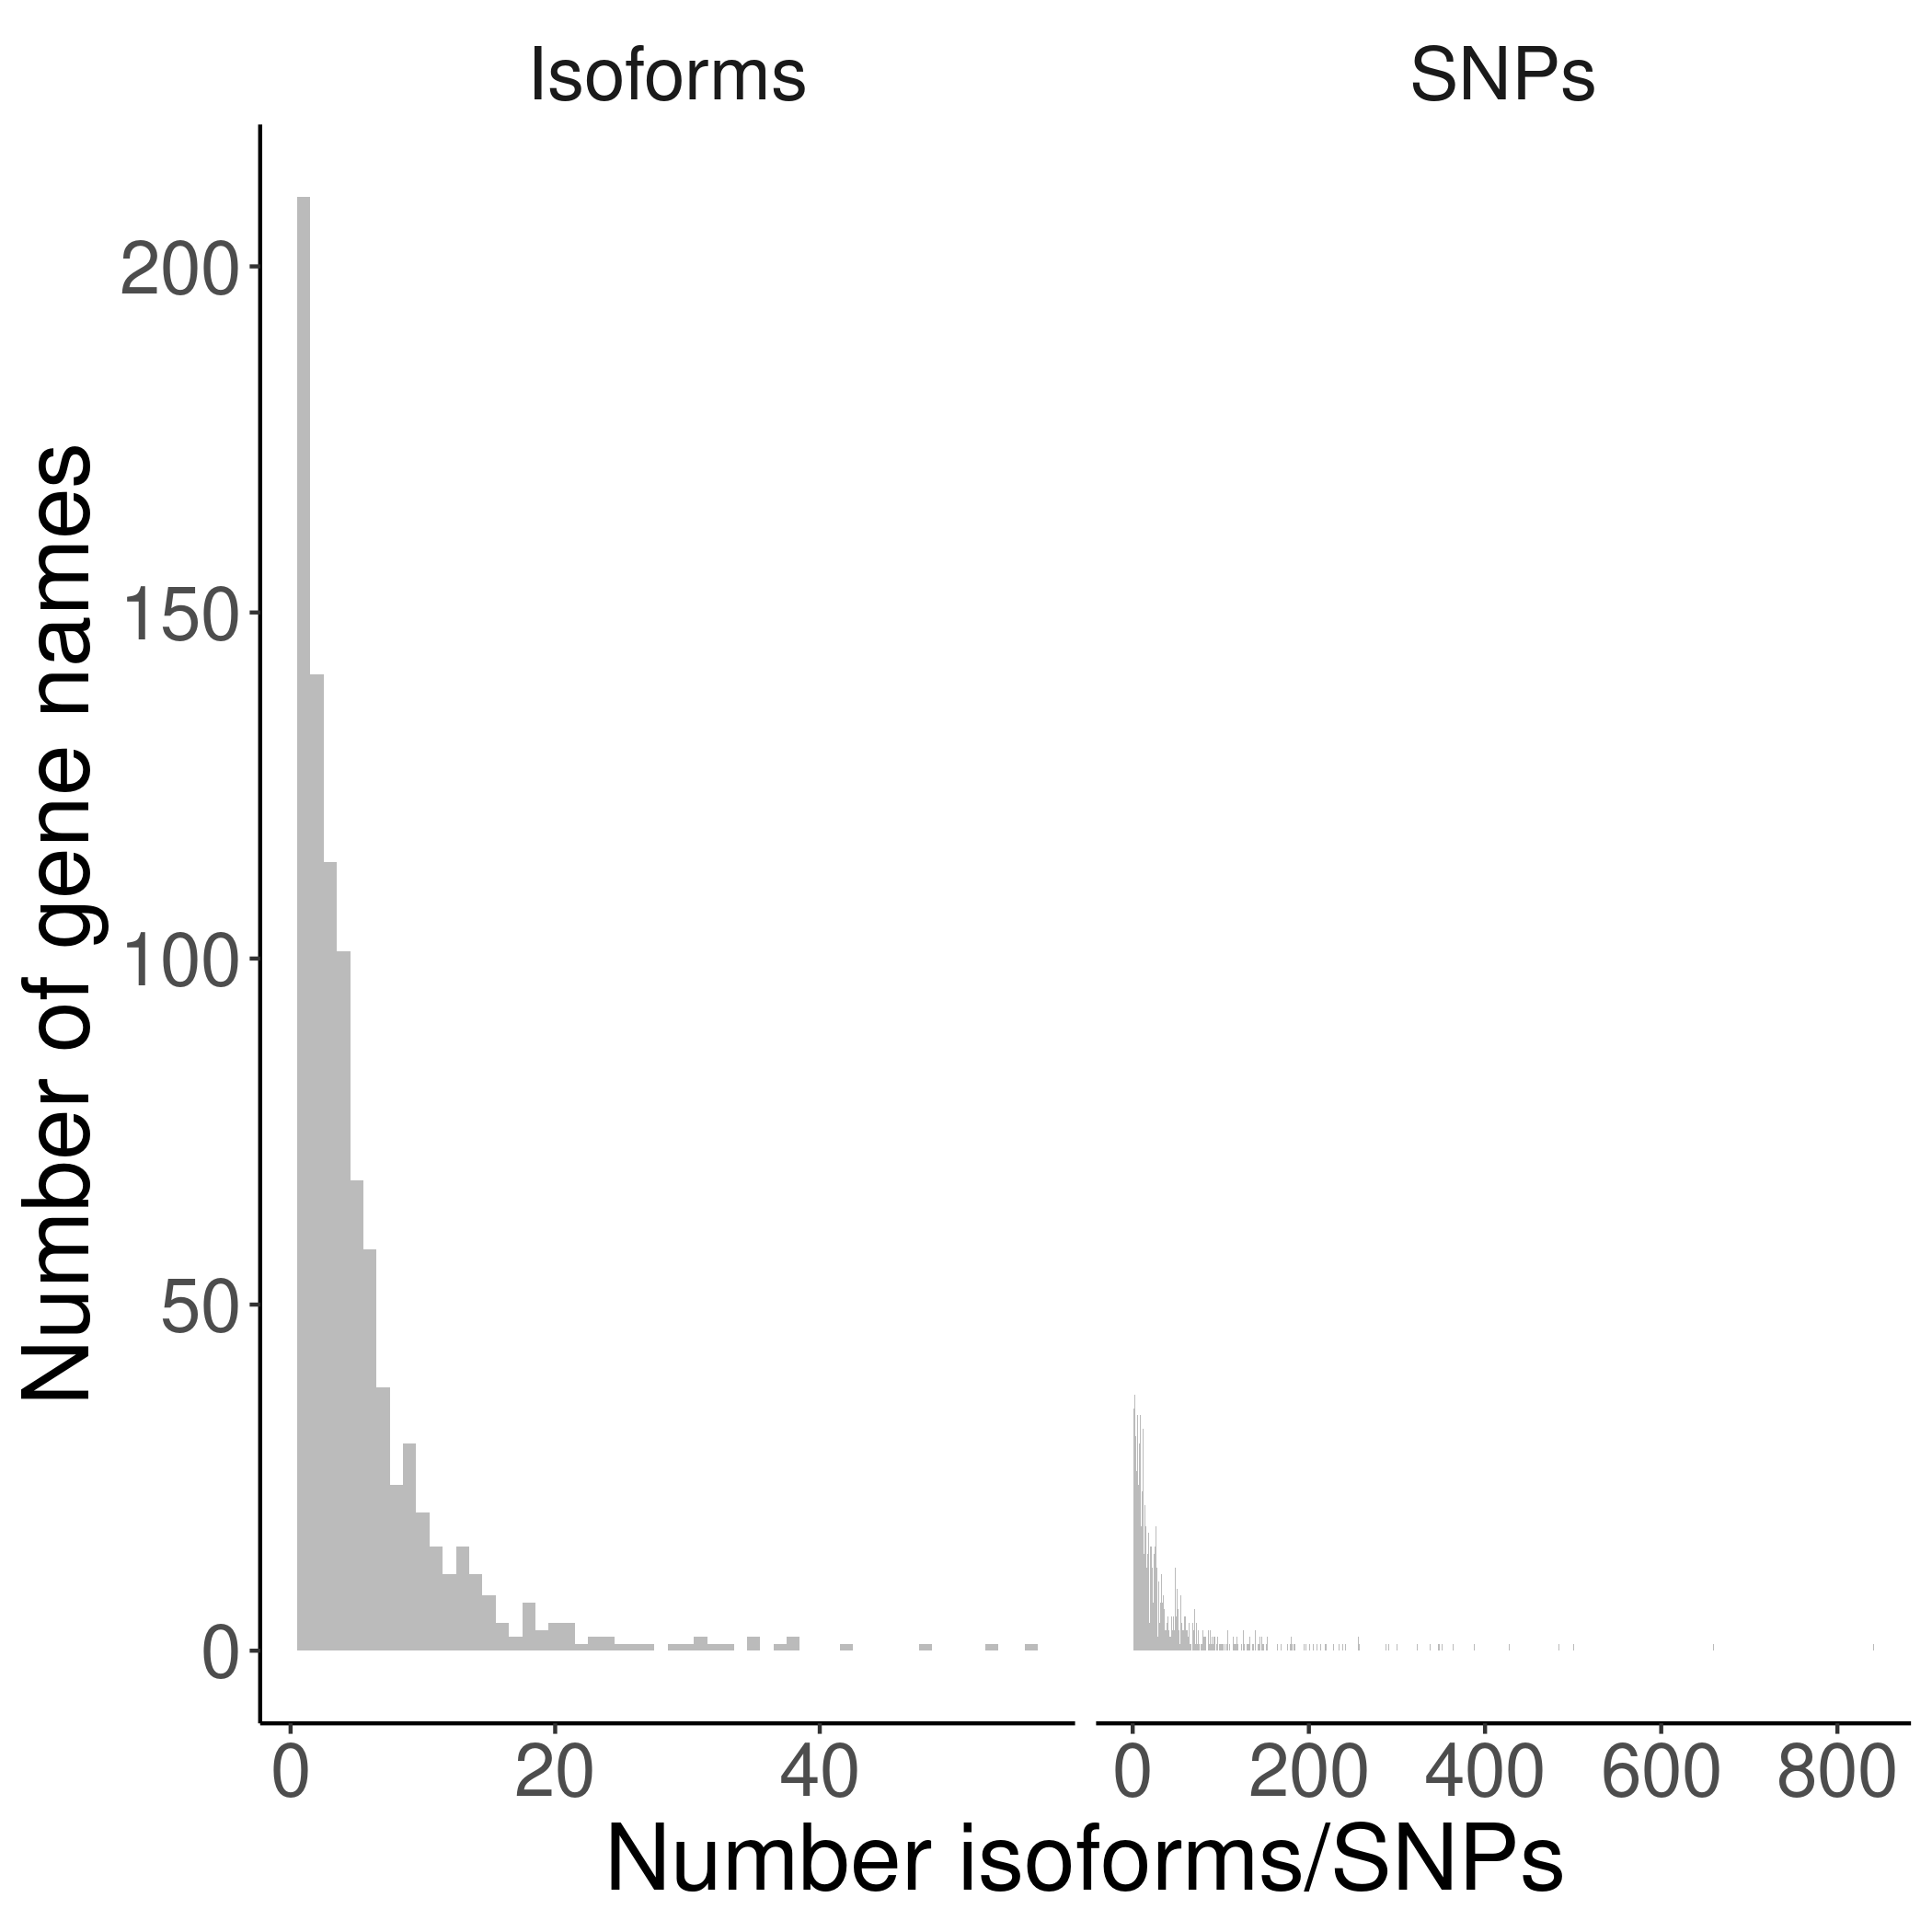
\includegraphics[width=\textwidth]{ncbi_peregrine_results/fig_n_proteins_per_gene_name.png}
  \caption{
    Histogram of the number of proteins found per gene name.
    Most often, a gene name is associated with one proteins. 
  }
  \label{fig:n_proteins_per_gene_name}
\end{figure}

\begin{figure}[!htbp]
  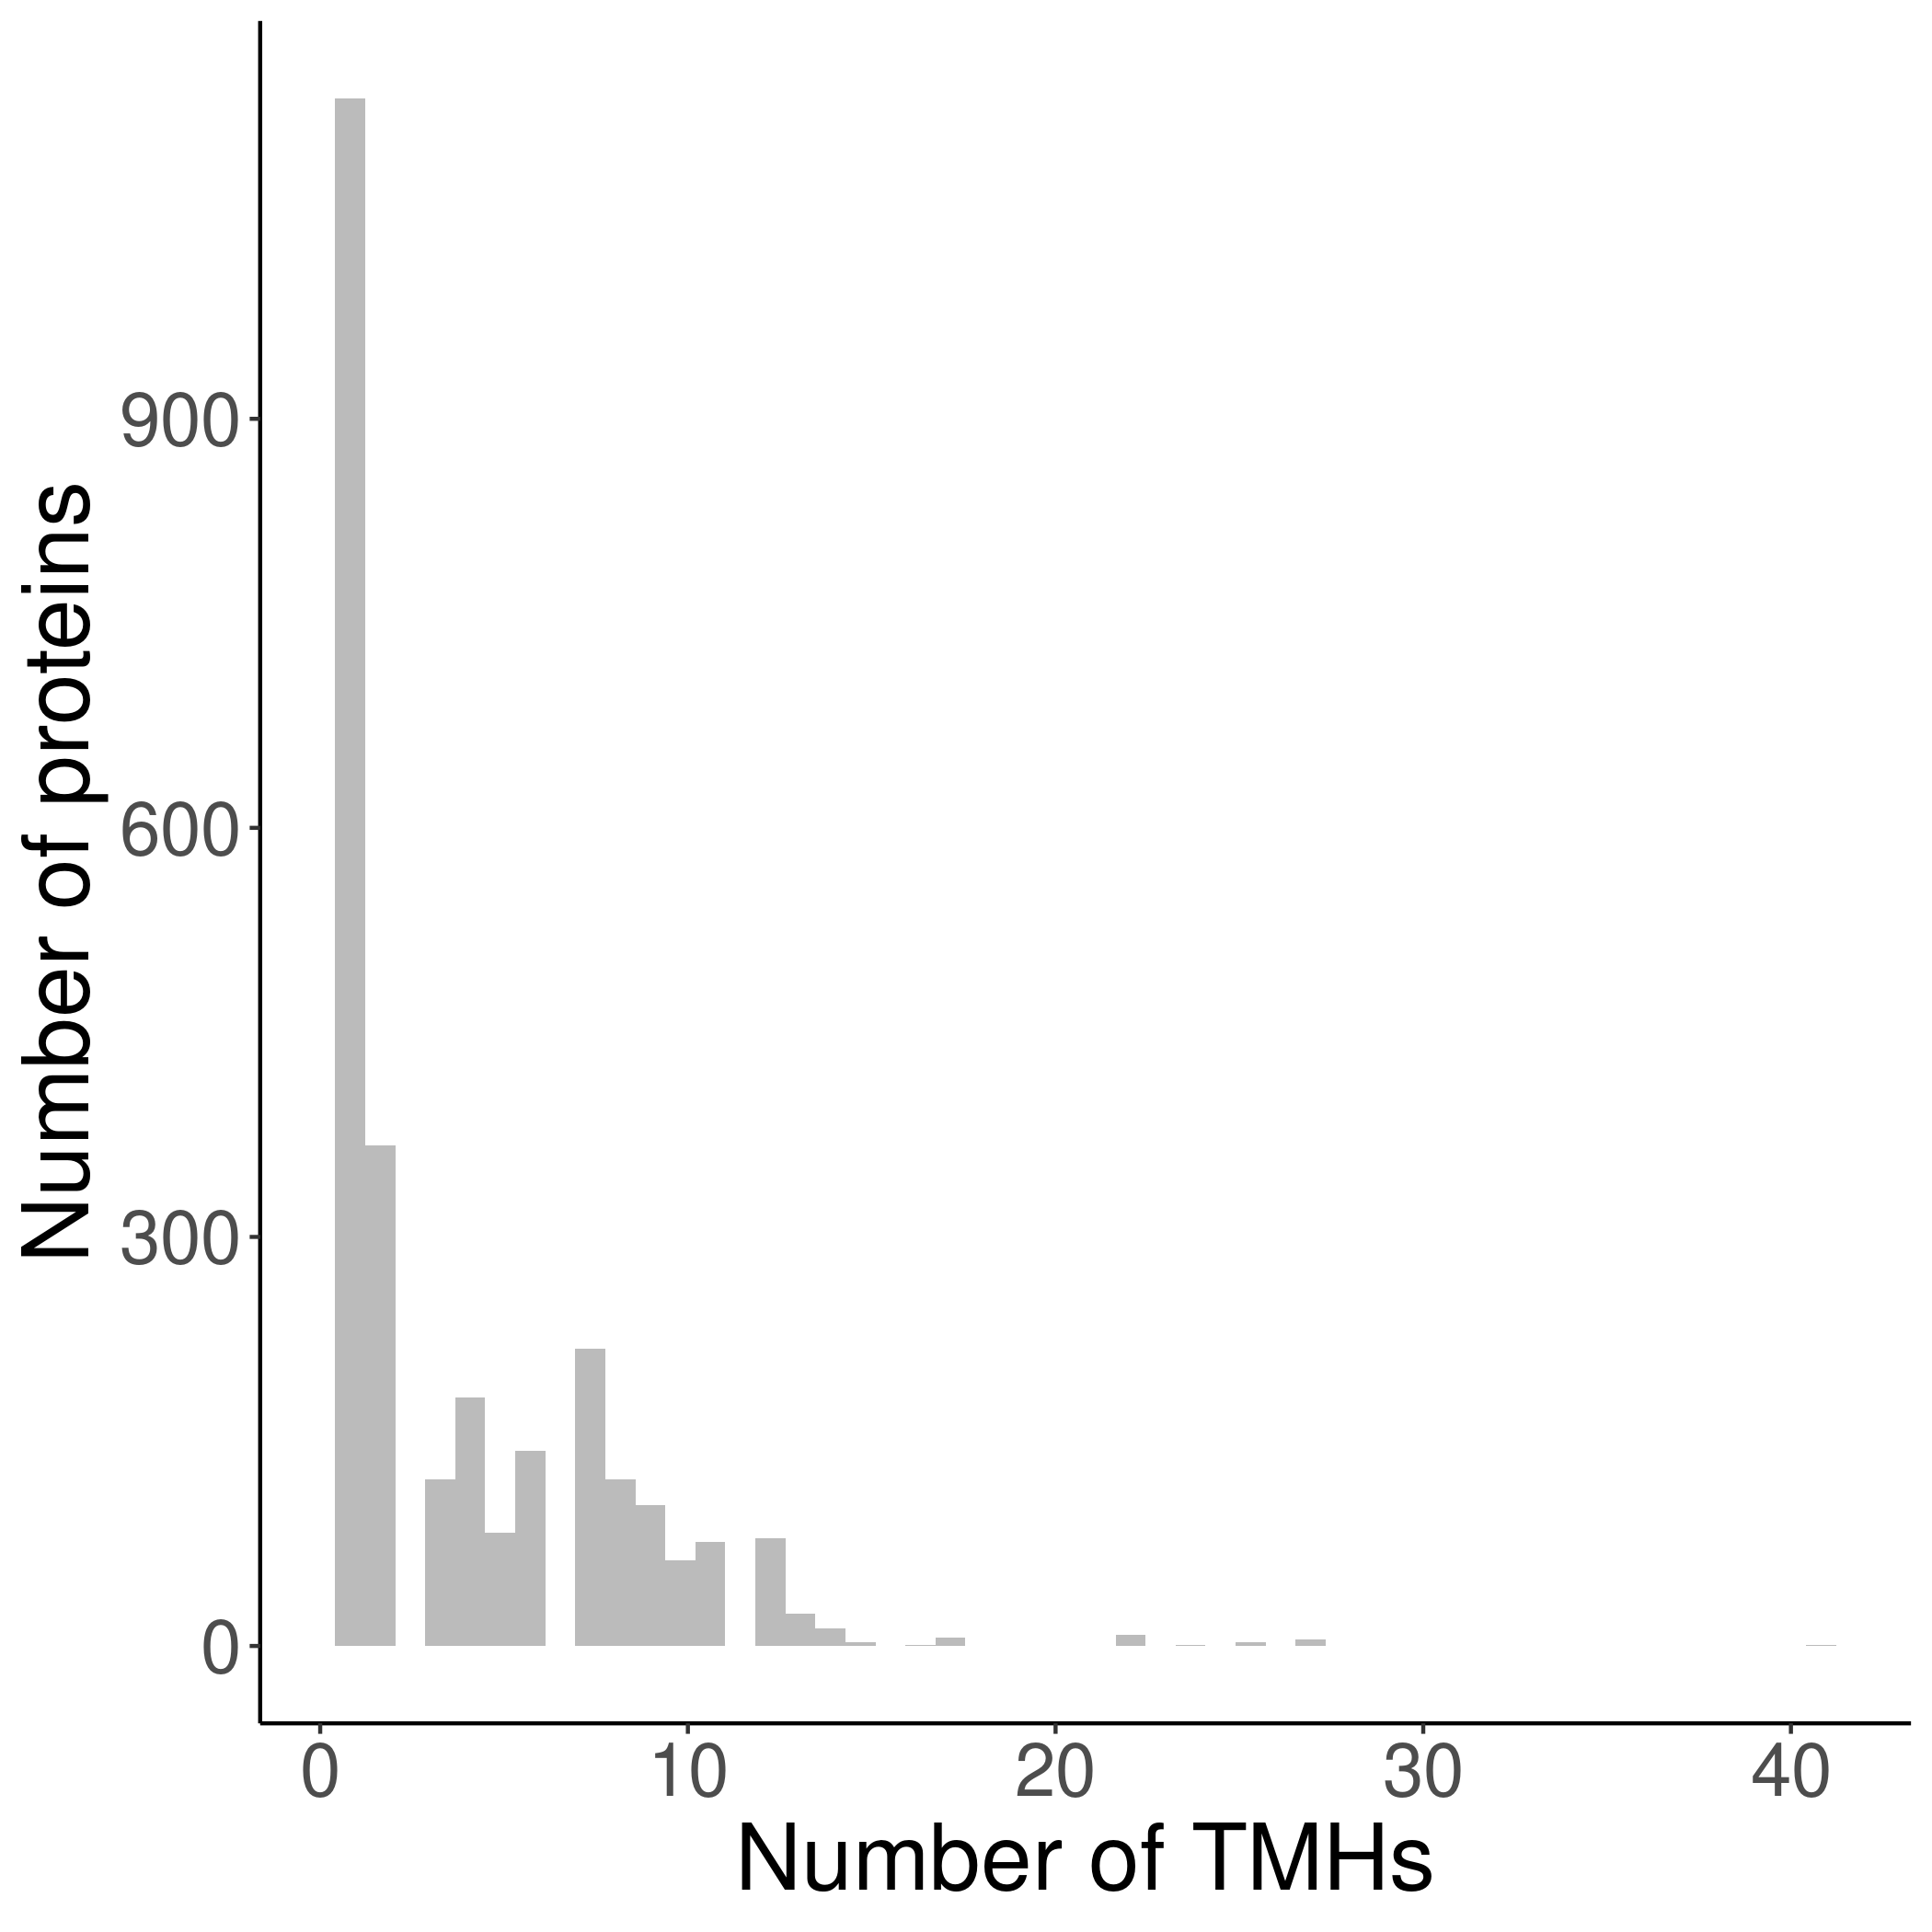
\includegraphics[width=\textwidth]{ncbi_peregrine_results/fig_n_tmhs_per_protein.png}
  \caption{
    Histogram of the number of TMHs predicted per protein,
    for the integral membrane proteins used.
  }
  \label{fig:n_tmhs_per_protein}
\end{figure}

\begin{figure}[!htbp]
  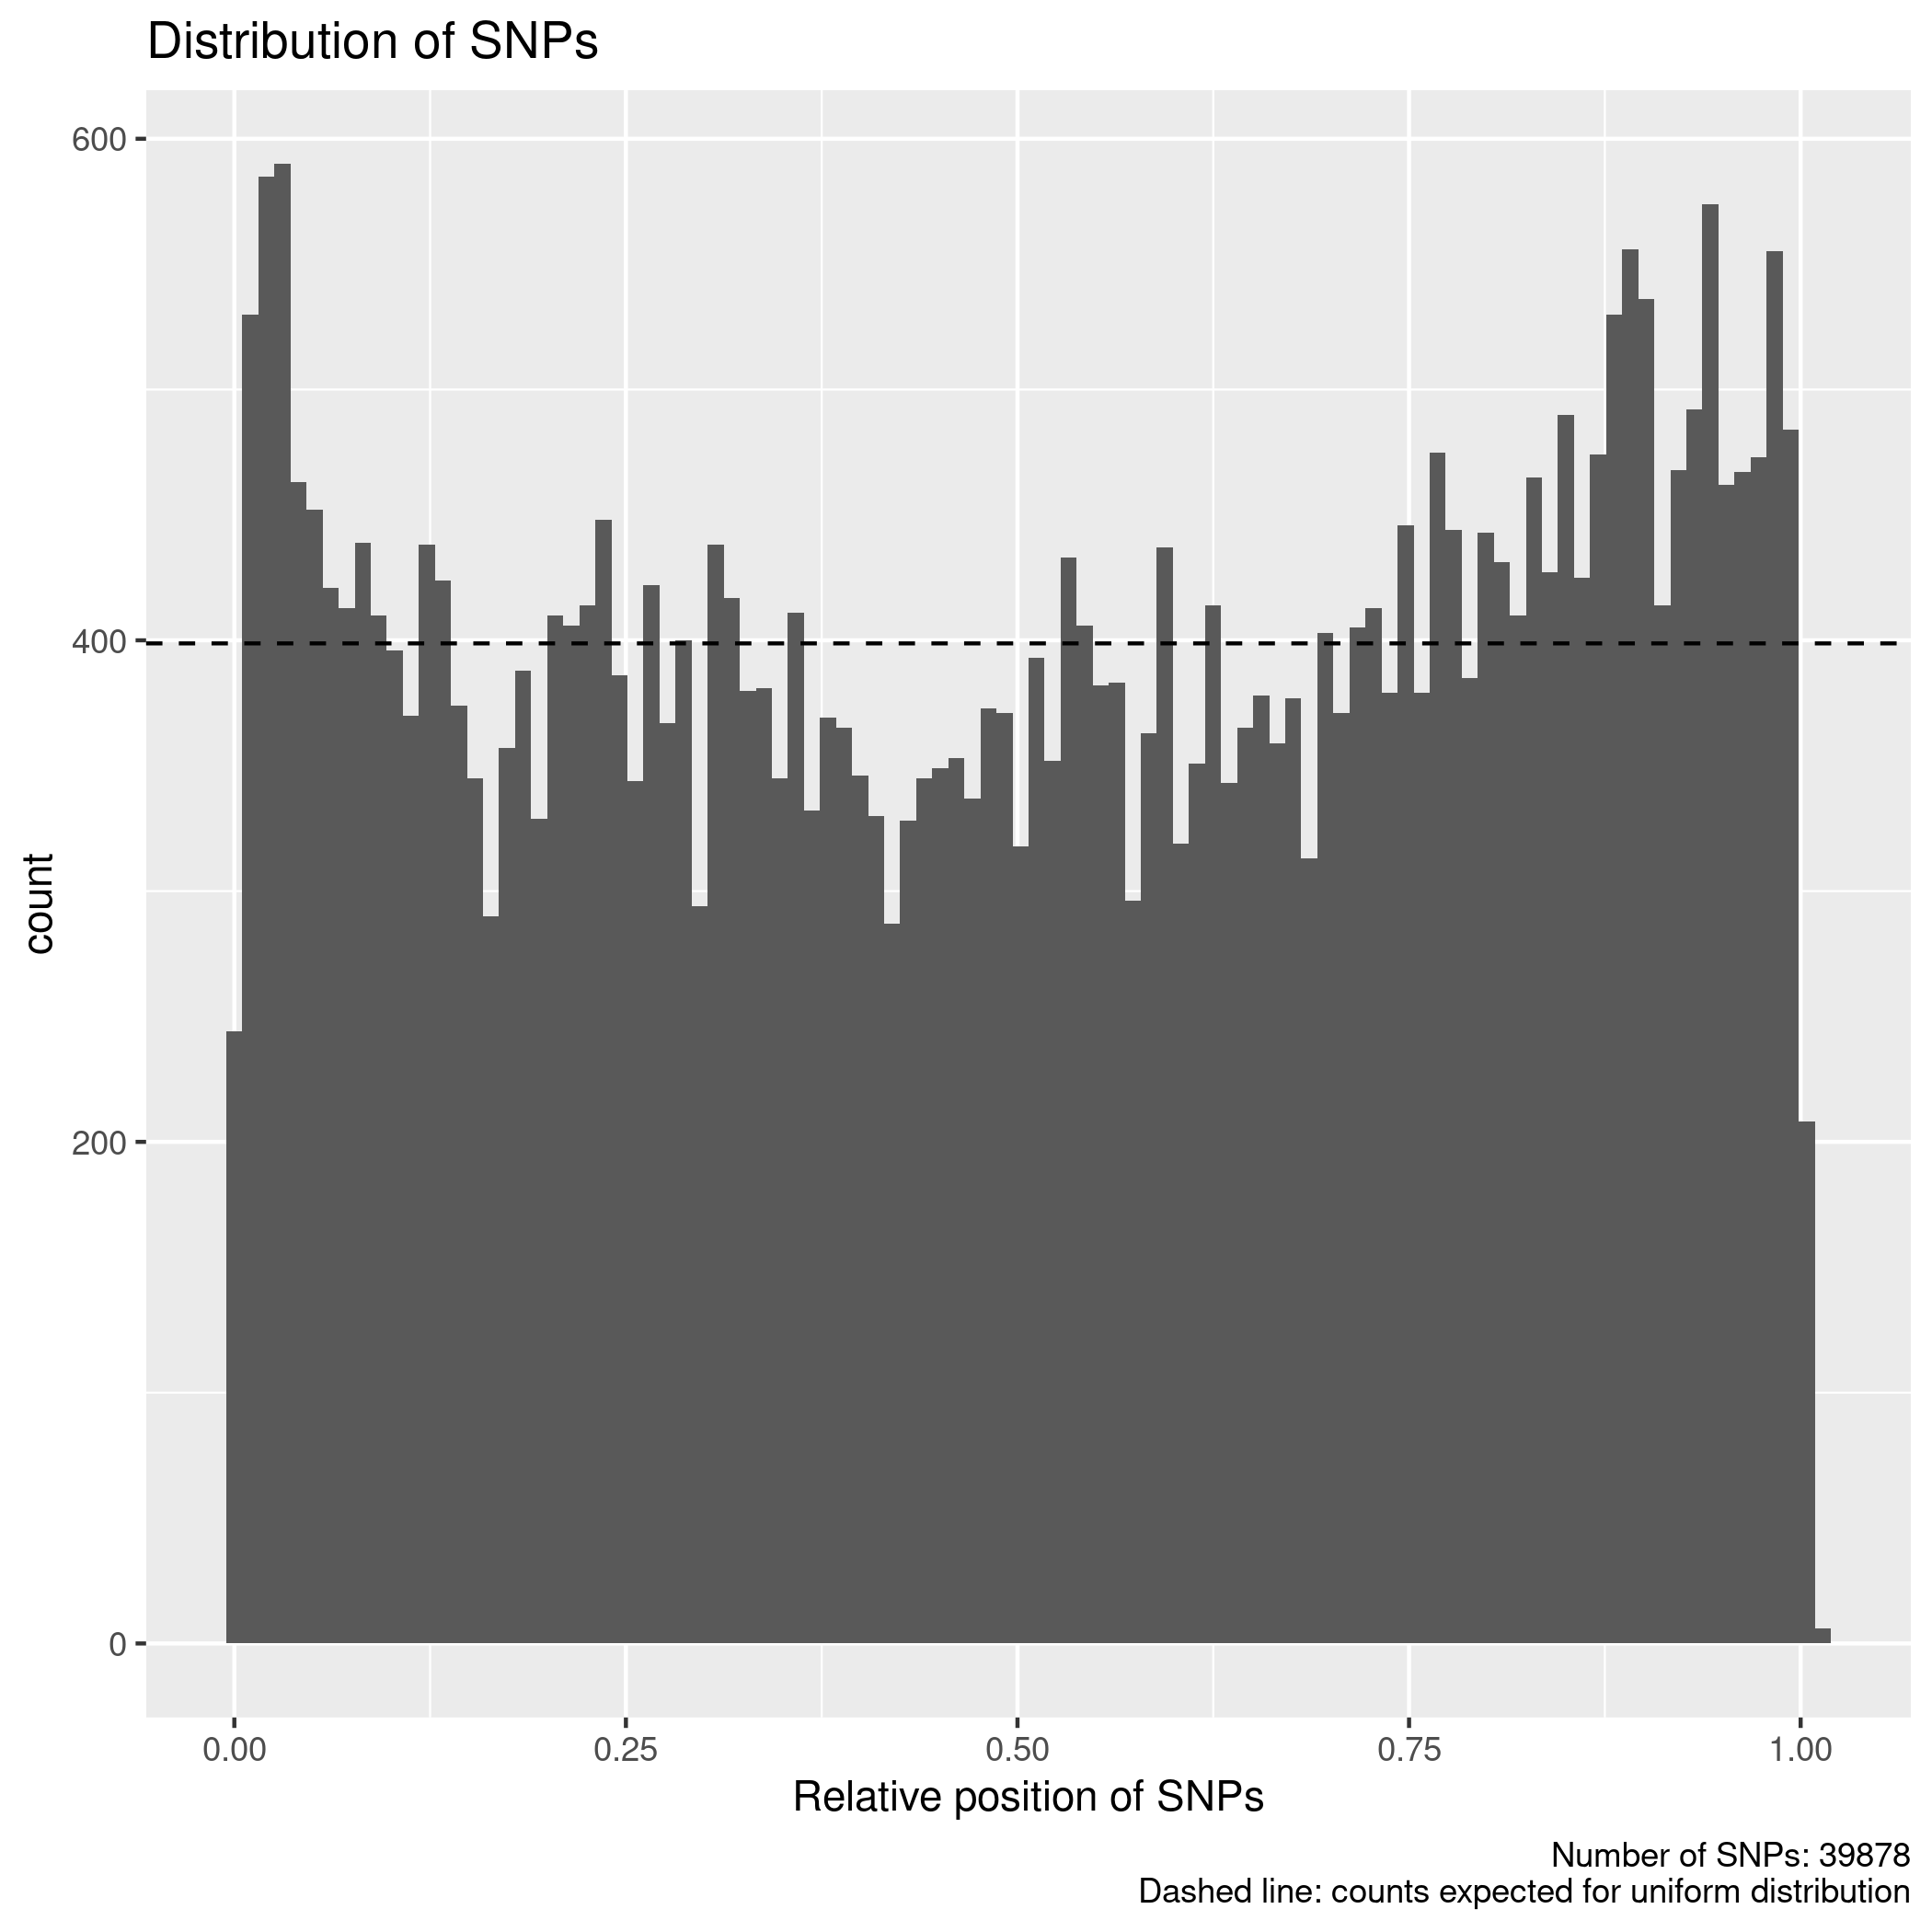
\includegraphics[width=\textwidth]{ncbi_peregrine_results/fig_snp_rel_pos.png}
  \caption{
    Distribution of the relative position of the SNPs used,
    where a relative position of zero denotes the first amino
    acid at the N-terminus, where a relative position of one
    indicates the last residue at the C-terminus.
  }
  \label{fig:snp_rel_pos}
\end{figure}

%
% Notes to self
%

%\begin{sidewaystable}
%  \centering
%  ... centered table here
%\end{sidewaystable}

% \scalebox{0.7}{
%  ... scaled table here
% }

%{\tiny
%  ... something with a tiny font
%}

% Instead of non-TMH use 'soluble protein region'
% or 'cytosolic or extracellular protein region'

